% Informe del proyecto de análisis semántico de Compiscript.
% Compilar con: tectonic -X compile informe.tex
\documentclass[11pt,a4paper]{article}

\usepackage[T1]{fontenc}
\usepackage{lmodern}
\usepackage[spanish,es-tabla,es-noquoting]{babel}
\usepackage[margin=2.5cm]{geometry}
\usepackage{graphicx}
\usepackage{xcolor}
\usepackage{booktabs}
\usepackage{longtable}
\usepackage{array}
\usepackage{tabularx}
\usepackage{listings}
\usepackage{caption}
\usepackage{float}
\usepackage{enumitem}
\usepackage{fancyhdr}
\usepackage[hidelinks]{hyperref}

\definecolor{fondoCodigo}{RGB}{247,248,250}
\definecolor{bordeCodigo}{RGB}{200,205,214}
\definecolor{comentario}{RGB}{95,120,95}
\definecolor{palabraClave}{RGB}{40,70,150}
\definecolor{cadena}{RGB}{150,60,40}
\definecolor{verdeUVG}{RGB}{0,105,60}

\lstdefinelanguage{Compiscript}{
  morekeywords={let,const,var,function,class,new,this,return,if,else,while,
    do,for,foreach,in,break,continue,switch,case,default,try,catch,print,
    integer,float,string,boolean,void,null,true,false},
  sensitive=true,
  morecomment=[l]{//},
  morecomment=[s]{/*}{*/},
  morestring=[b]",
}

\lstset{
  basicstyle=\ttfamily\footnotesize,
  keywordstyle=\color{palabraClave}\bfseries,
  commentstyle=\color{comentario}\itshape,
  stringstyle=\color{cadena},
  backgroundcolor=\color{fondoCodigo},
  frame=single,
  rulecolor=\color{bordeCodigo},
  breaklines=true,
  showstringspaces=false,
  extendedchars=true,
  numbers=left,
  numberstyle=\tiny\color{gray},
  numbersep=8pt,
  xleftmargin=18pt,
  framexleftmargin=18pt,
  captionpos=b,
}

\pagestyle{fancy}
\fancyhf{}
\fancyhead[L]{\small Fase de Compilación: Análisis Semántico}
\fancyhead[R]{\small Compiscript --- ANTLR + C++}
\fancyfoot[C]{\thepage}
\renewcommand{\headrulewidth}{0.4pt}

\captionsetup{font=small,labelfont=bf}
\setlength{\parskip}{0.5em}
\setlength{\parindent}{0pt}

\newcolumntype{L}[1]{>{\raggedright\arraybackslash}p{#1}}

\begin{document}

% ------------------------------------------------------------------ CARÁTULA
\begin{titlepage}
\begin{center}

\vspace*{0.2cm}


\includegraphics[width=0.24\textwidth]{img/uvg-logo.png}

\vspace{0.8cm}

{\Large\scshape Universidad del Valle de Guatemala}\\[0.30cm]
{\large Facultad de Ingeniería}\\[0.20cm]
{\large Departamento de Ciencias de la Computación}\\[0.20cm]
{\large Construcción de Compiladores}

\vspace{1.1cm}

\rule{\textwidth}{0.8pt}

\vspace{0.5cm}

{\Huge\bfseries Fase de Compilación:}\\[0.30cm]
{\Huge\bfseries Análisis Semántico}

\vspace{0.5cm}

{\Large Analizador sintáctico y semántico de Compiscript}\\[0.30cm]
{\footnotesize\url{https://github.com/G1LB3T0/Proyecto1_Compis_Generador_Analizador_Lexico/tree/compiladores-2}}

\vspace{0.5cm}

\rule{\textwidth}{0.8pt}

\vspace{1.2cm}

{\large\bfseries Catedrático}\\[0.25cm]
{\large Ing. Pablo Koch}

\vspace{0.9cm}

{\large\bfseries Integrantes}\\[0.3cm]
{\large Luis Gonzalez --- 23353}\\[0.2cm]
{\large Joel Jaquez --- 23369}

\vfill

{\large Guatemala, 6 de septiembre de 2026}

\end{center}
\end{titlepage}

\tableofcontents
\newpage

% ------------------------------------------------------------ 1 INTRODUCCIÓN
\section{Introducción}

Este informe documenta la implementación del analizador sintáctico y semántico
de \textbf{Compiscript}, un lenguaje basado en un subconjunto de TypeScript. El
trabajo corresponde a la fase de análisis semántico en la construcción de un
compilador: partiendo de la gramática oficial en ANTLR se construye el árbol
sintáctico, se recorre mediante un \emph{Visitor} y se validan las reglas de
tipos, ámbitos, funciones, control de flujo, clases y estructuras de datos,
sosteniendo en todo momento una tabla de símbolos con entornos anidados.

La característica que distingue esta implementación es que \textbf{todo el
compilador está escrito en C++17}. ANTLR se utilizó con su \emph{target} de C++,
de modo que el lexer, el parser y el visitor generados se compilan y enlazan
junto con el analizador semántico en una sola biblioteca nativa. Python aparece
únicamente como adaptador web: un servidor Flask de 139 líneas que sirve el IDE
y traduce peticiones HTTP en invocaciones al ejecutable C++. Ninguna regla
léxica, sintáctica o semántica está implementada en Python ni en JavaScript.

El sistema acepta archivos con extensión \texttt{.cps} y produce, en un único
documento JSON, la lista de tokens, el árbol sintáctico serializado, los
diagnósticos con ubicación exacta y el estado completo de la tabla de símbolos
por cada entorno creado.

% -------------------------------------------------------------- 2 OBJETIVOS
\section{Objetivos}

\subsection{Objetivo general}

Implementar un analizador semántico funcional para Compiscript, aplicando los
conceptos de sistemas de tipos, ámbitos y entornos de ejecución sobre un árbol
sintáctico real, con una tabla de símbolos capaz de sostener las fases
posteriores del compilador.

\subsection{Objetivos específicos}

\begin{itemize}[leftmargin=1.4em]
  \item Implementar el analizador sintáctico de Compiscript utilizando ANTLR.
  \item Construir el árbol sintáctico con representación visual navegable.
  \item Recorrer el árbol mediante un \emph{Visitor} de ANTLR para evaluar las
        reglas semánticas del lenguaje.
  \item Implementar una batería de pruebas que valide casos exitosos y fallidos
        para cada regla semántica.
  \item Desarrollar un IDE que permita escribir, cargar y compilar código
        Compiscript.
\end{itemize}

% ------------------------------------------------------------ 3 ARQUITECTURA
\section{Arquitectura general}

\subsection{El pipeline}

El flujo de información va del texto fuente al documento JSON que consume el
IDE. Cada etapa tiene una responsabilidad única y un artefacto de salida
observable:

\begin{center}
\begin{minipage}{0.86\textwidth}
\ttfamily\small
\begin{verbatim}
Código .cps
    |
    v
CompiscriptLexer  (ANTLR, C++)
    | tokens
    v
CompiscriptParser (ANTLR, C++)
    | parse tree
    |---------------> tree_serializer -> árbol JSON -> IDE
    |
    v
SemanticAnalyzer  (Visitor C++, deriva de CompiscriptBaseVisitor)
    |
    |-- sistema de tipos y compatibilidad
    |-- resolución léxica de nombres (tabla de símbolos)
    |-- funciones, recursión y closures
    |-- control de flujo y código muerto
    |-- clases, herencia, miembros y constructores
    |-- listas e índices
    |
    v
JSON: diagnósticos + scopes + símbolos + clases
    |
    v
Flask (adaptador) -> IDE web
\end{verbatim}
\end{minipage}
\end{center}

\subsection{Núcleo independiente de la interfaz}

El núcleo C++ expone una sola función pública, \texttt{analyzeSource}, que
recibe el texto del programa y devuelve un \texttt{AnalysisResult}. Los tres
consumidores del sistema ---el CLI, la batería de pruebas y el servidor
Flask--- utilizan esa misma API. Esta decisión evita el problema clásico de
tener implementaciones divergentes del compilador para la línea de comandos y
para la interfaz gráfica: lo que prueba la batería es exactamente lo que
ejecuta el IDE.

Otra decisión relevante es que \textbf{el análisis semántico no se ejecuta
cuando existen errores léxicos o sintácticos}. Recorrer un árbol recuperado e
incompleto produce diagnósticos en cascada que confunden más de lo que ayudan.
Aun así, los tokens y el árbol se conservan y se envían al IDE, porque son
justamente la información que el usuario necesita para corregir la entrada.

% ------------------------------------------------- 4 TRAZABILIDAD POR COMMITS
\section{Estructura del repositorio y trazabilidad por commits}

El desarrollo de esta fase se realizó en la rama \texttt{compiladores-2}. Cada
commit corresponde a una unidad funcional completa y a un solo autor, de modo
que la contribución individual queda registrada en el historial. En Git se
utilizaron tres identidades que corresponden a los dos integrantes:

\begin{table}[H]
\centering
\small
\begin{tabular}{lll}
\toprule
\textbf{Identidad en Git} & \textbf{Correo} & \textbf{Integrante} \\
\midrule
\texttt{G1LB3T0}      & luis.yo09@hotmail.com   & Luis Gonzalez (23353) \\
\texttt{jaq23369}     & jaq23369@uvg.edu.gt     & Joel Jaquez (23369) \\
\texttt{Joel Jaquez}  & 123708276+jaq23369@\dots & Joel Jaquez (23369) \\
\bottomrule
\end{tabular}
\caption{Identidades de Git utilizadas en la rama.}
\end{table}

\subsection{Historial de la rama}

La tabla siguiente recorre los ocho commits de la rama en orden cronológico y
explica qué archivos introduce cada uno y por qué. Es, en la práctica, el mapa
de lectura del repositorio.

\begin{longtable}{@{}p{1.6cm}L{2.7cm}L{9.1cm}@{}}
\toprule
\textbf{Commit} & \textbf{Autor} & \textbf{Aporte y archivos} \\
\midrule
\endfirsthead
\toprule
\textbf{Commit} & \textbf{Autor} & \textbf{Aporte y archivos} \\
\midrule
\endhead

\texttt{6de9fe5} & Joel Jaquez &
\textbf{[INIT] Preparar la base del proyecto Compiscript.} Incorpora el material
oficial en \texttt{Instrucciones/}: el enunciado, la especificación del lenguaje
y la gramática entregada \texttt{Compiscript (1).g4}. Ajusta
\texttt{.gitignore} y el \texttt{README.md} para separar el trabajo de esta fase
del de Compiladores 1. \\
\addlinespace

\texttt{ac9e6cf} & Luis Gonzalez &
\textbf{[ADD] Configurar ANTLR y compilación de Compiscript.} Es el commit que
levanta la infraestructura. Añade
\texttt{backend/compiscript/grammar/Compiscript.g4} (la gramática activa, ya
extendida), los doce archivos de
\texttt{backend/compiscript/generated/} producidos por ANTLR con el
\emph{target} de C++, el \texttt{CMakeLists.txt} que compila el runtime C++ de
ANTLR junto con el proyecto, y los scripts reproducibles
\texttt{scripts/build\_compiscript.sh}, \texttt{.ps1} y
\texttt{generate\_antlr.sh}. \\
\addlinespace

\texttt{dafd076} & Joel Jaquez &
\textbf{[ADD] Implementar análisis semántico de Compiscript.} El corazón del
proyecto. Introduce \texttt{include/compiscript/model.h} (símbolos, scopes y
clases), \texttt{include/compiscript/semantic\_analyzer.h} y las 1\,218 líneas
de \texttt{src/semantic\_analyzer.cpp}, que es el Visitor propiamente dicho,
más \texttt{src/symbol\_table.cpp} con la mecánica de declaración y resolución
de nombres. \\
\addlinespace

\texttt{f911f64} & Luis Gonzalez &
\textbf{[ADD] Integrar servicio C++ y salida del analizador.} Convierte el
Visitor en un servicio consumible. Añade \texttt{service.\{h,cpp\}}
(orquestación del pipeline y \texttt{analyzeSource}),
\texttt{diagnostics.\{h,cpp\}} (código estable, categoría, severidad, línea y
columna), \texttt{tree\_serializer.\{h,cpp\}} (parse tree $\rightarrow$ JSON),
\texttt{token\_classifier.\{h,cpp\}} (categoría legible de cada token),
\texttt{json.\{h,cpp\}} (serialización sin dependencias externas) y
\texttt{main.cpp}, el ejecutable \texttt{compiscript\_cli}. \\
\addlinespace

\texttt{a1ffefe} & Joel Jaquez &
\textbf{[ADD] Desarrollar IDE de análisis para Compiscript.} Construye la
interfaz: \texttt{frontend/templates/index.html},
\texttt{frontend/static/js/app.js} (1\,001 líneas: editor, árbol interactivo,
tablas y navegación de diagnósticos), \texttt{frontend/static/css/style.css},
el adaptador \texttt{app.py} y \texttt{requirements.txt}. \\
\addlinespace

\texttt{49af6b1} & Luis Gonzalez &
\textbf{[TEST] Cubrir reglas semánticas de Compiscript.} Añade
\texttt{backend/tests/compiscript\_tests.cpp} (654 líneas, 95 escenarios) y los
tres programas de demostración
\texttt{backend/examples/compiscript/}: \texttt{bienvenido.cps},
\texttt{closures.cps} y \texttt{errores\_semanticos.cps}. \\
\addlinespace

\texttt{a40593a} & Joel Jaquez &
\textbf{[DOC] Documentar arquitectura y evaluación de Compiscript.} Crea
\texttt{docs/arquitectura-compiscript.md} y
\texttt{docs/decisiones-compiscript.md}, reescribe el \texttt{README.md} y
elimina archivos de planificación que ya no correspondían al estado del
proyecto. \\
\addlinespace

\texttt{12bfe89} & Joel Jaquez &
\textbf{[ADD] Comentarios importantes.} Pasada final de documentación en el
código: comenta los 25 archivos fuente del núcleo, las pruebas, el frontend y
los scripts, explicando la intención de cada módulo. \\
\bottomrule
\caption{Trazabilidad de la rama \texttt{compiladores-2}.}
\end{longtable}

\subsection{Lectura del historial}

El orden de los commits refleja el orden natural de construcción de un
compilador y conviene leerlo así: primero la gramática y la generación
(\texttt{ac9e6cf}), luego el Visitor que da significado al árbol
(\texttt{dafd076}), después la capa que expone los resultados
(\texttt{f911f64}), sobre ella la interfaz (\texttt{a1ffefe}), y finalmente la
evidencia de que todo lo anterior funciona (\texttt{49af6b1}) y la explicación
de por qué está hecho así (\texttt{a40593a}, \texttt{12bfe89}).

% -------------------------------------------------- 5 ARCHIVOS POR CAPA
\section{Descripción de los archivos por capa}

\subsection{Capa de gramática y código generado}

\begin{table}[H]
\centering
\small
\begin{tabular}{@{}L{6.3cm}rL{6.3cm}@{}}
\toprule
\textbf{Archivo} & \textbf{Líneas} & \textbf{Función} \\
\midrule
\texttt{grammar/Compiscript.g4} & 115 &
Fuente de verdad sintáctica. Define tokens y reglas del lenguaje. \\
\texttt{generated/CompiscriptLexer.*} & --- &
Autómata léxico generado por ANTLR. \\
\texttt{generated/CompiscriptParser.*} & --- &
Parser ALL(*) y contextos de regla. \\
\texttt{generated/CompiscriptVisitor.*} & --- &
Interfaz del patrón Visitor. \\
\texttt{generated/CompiscriptBaseVisitor.*} & --- &
Implementación por defecto de la que hereda el analizador. \\
\bottomrule
\end{tabular}
\caption{Archivos de la capa sintáctica.}
\end{table}

El código generado se versiona en el repositorio a propósito: permite compilar
el proyecto sin Java disponible, mientras que los scripts permiten regenerarlo
cuando la gramática cambia.

\subsection{Núcleo del analizador}

\begin{table}[H]
\centering
\small
\begin{tabular}{@{}L{6.3cm}rL{6.3cm}@{}}
\toprule
\textbf{Archivo} & \textbf{Líneas} & \textbf{Función} \\
\midrule
\texttt{src/semantic\_analyzer.cpp} & 1218 &
El Visitor. Sintetiza tipos, aplica reglas contextuales y emite diagnósticos. \\
\texttt{include/.../model.h} & 127 &
Estructuras \texttt{Symbol}, \texttt{Scope}, \texttt{ClassInfo} y
\texttt{AnalysisResult}. \\
\texttt{include/.../semantic\_analyzer.h} & 171 &
Declaración del Visitor y su estado contextual. \\
\texttt{src/json.cpp} & 225 &
Serializador JSON propio, sin dependencias externas. \\
\texttt{src/service.cpp} & 76 &
Orquesta lexer, parser, serializador y Visitor. \\
\texttt{src/tree\_serializer.cpp} & 68 &
Convierte el parse tree de ANTLR en JSON recursivo. \\
\texttt{src/token\_classifier.cpp} & 65 &
Asigna categoría legible a cada token. \\
\texttt{src/main.cpp} & 53 &
Ejecutable \texttt{compiscript\_cli}. \\
\texttt{src/symbol\_table.cpp} & 38 &
Declaración y resolución de nombres en la cadena de ámbitos. \\
\texttt{src/diagnostics.cpp} & 21 &
Construcción uniforme de diagnósticos. \\
\bottomrule
\end{tabular}
\caption{Archivos del núcleo C++.}
\end{table}

\subsection{Pruebas, IDE y construcción}

\begin{table}[H]
\centering
\small
\begin{tabular}{@{}L{6.3cm}rL{6.3cm}@{}}
\toprule
\textbf{Archivo} & \textbf{Líneas} & \textbf{Función} \\
\midrule
\texttt{tests/compiscript\_tests.cpp} & 654 &
95 escenarios enlazados contra \texttt{compiscript\_core}. \\
\texttt{frontend/static/js/app.js} & 1001 &
Editor, árbol interactivo, tablas y navegación de errores. \\
\texttt{frontend/static/css/style.css} & 235 & Hoja de estilos del IDE. \\
\texttt{frontend/templates/index.html} & 101 & Estructura de la interfaz. \\
\texttt{app.py} & 139 & Adaptador Flask. Cuatro endpoints. \\
\texttt{CMakeLists.txt} & --- &
Compila el runtime de ANTLR, la biblioteca, el CLI y las pruebas. \\
\texttt{scripts/build\_compiscript.*} & --- &
Descarga ANTLR, regenera, compila y ejecuta la batería. \\
\bottomrule
\end{tabular}
\caption{Archivos de pruebas, interfaz y construcción.}
\end{table}

El servidor expone cuatro endpoints: \texttt{/api/files} y
\texttt{/api/file/<nombre>} para listar y leer ejemplos, \texttt{/api/save}
para guardar, \texttt{/api/analyze} que ejecuta \texttt{compiscript\_cli} con la
fuente por entrada estándar, y \texttt{/api/tests} que ejecuta el binario de la
batería. En los dos últimos casos Flask se limita a reenviar el JSON producido
por C++.

% ----------------------------------------------------------- 6 GRAMÁTICA
\section{Gramática y generación con ANTLR}

La gramática activa reside en
\texttt{backend/compiscript/grammar/Compiscript.g4} y se genera con el
\emph{target} de C++ y el patrón Visitor:

\begin{lstlisting}[language=bash,caption={Generación del lexer, parser y Visitor.}]
java -jar tools/antlr-4.13.2-complete.jar -Dlanguage=Cpp -visitor \
     -no-listener -o backend/compiscript/generated -Xexact-output-dir \
     Compiscript.g4
\end{lstlisting}

Se eligió \emph{Visitor} y no \emph{Listener} porque el análisis semántico
necesita \textbf{sintetizar} valores: el tipo de una expresión se obtiene a
partir del tipo de sus subexpresiones, y el Visitor permite que cada
\texttt{visitX} devuelva ese tipo hacia el nodo padre. Con un Listener habría
que mantener manualmente una pila de resultados.

% ------------------------------------------------------ 7 REGLAS SEMÁNTICAS
\section{Reglas semánticas implementadas}

El Visitor emite 32 códigos de diagnóstico distintos, todos con categoría,
severidad, línea y columna. La tabla siguiente los agrupa por la familia de
reglas que exige el enunciado.

\begin{longtable}{@{}p{3.6cm}L{11.4cm}@{}}
\toprule
\textbf{Familia} & \textbf{Comportamiento implementado y códigos} \\
\midrule
\endfirsthead
\toprule
\textbf{Familia} & \textbf{Comportamiento implementado y códigos} \\
\midrule
\endhead

Sistema de tipos &
Verifica \texttt{+}, \texttt{-}, \texttt{*}, \texttt{/} y \texttt{\%} sobre
números; \texttt{\&\&}, \texttt{||} y \texttt{!} sobre booleanos; comparaciones
compatibles; tipos de asignación; e inicialización obligatoria de
\texttt{const}. Reconoce \texttt{integer}, \texttt{float}, \texttt{string},
\texttt{boolean}, \texttt{null}, \texttt{void}, clases y listas, con ampliación
segura \texttt{integer} $\rightarrow$ \texttt{float}.
\newline
\texttt{SEM\_ARITHMETIC\_TYPE}, \texttt{SEM\_LOGICAL\_TYPE},
\texttt{SEM\_COMPARE\_TYPE}, \texttt{SEM\_ASSIGN\_TYPE},
\texttt{SEM\_ASSIGN\_CONST}, \texttt{SEM\_TERNARY\_TYPE},
\texttt{SEM\_TYPE\_UNKNOWN}, \texttt{SEM\_TYPE\_VOID}. \\
\addlinespace

Manejo de ámbito &
Resuelve primero el entorno local y continúa por los padres hasta el global;
reporta nombres no declarados y redeclaraciones; permite sombreado en entornos
hijos; crea un scope por programa, función, clase y bloque.
\newline
\texttt{SEM\_SCOPE\_UNDECLARED}, \texttt{SEM\_SCOPE\_DUPLICATE}. \\
\addlinespace

Funciones y procedimientos &
Conserva firmas completas, valida cantidad y tipo posicional de argumentos,
comprueba el tipo de retorno y los caminos sin retorno, admite recursión y
funciones anidadas, y registra las capturas de closures.
\newline
\texttt{SEM\_FUNCTION\_ARITY}, \texttt{SEM\_FUNCTION\_ARGUMENT},
\texttt{SEM\_FUNCTION\_RETURN}, \texttt{SEM\_FUNCTION\_MISSING\_RETURN},
\texttt{SEM\_FUNCTION\_NOT\_CALLABLE}. \\
\addlinespace

Control de flujo &
Exige condición booleana en \texttt{if}, \texttt{while}, \texttt{do-while},
\texttt{for} y \texttt{switch}; limita \texttt{break} y \texttt{continue} a
bucles y \texttt{return} a funciones; detecta instrucciones inalcanzables.
\newline
\texttt{SEM\_FLOW\_BREAK}, \texttt{SEM\_FLOW\_CONTINUE},
\texttt{SEM\_FLOW\_RETURN}, \texttt{SEM\_FLOW\_DEAD\_CODE},
\texttt{SEM\_SWITCH\_CASE}. \\
\addlinespace

Clases y objetos &
Comprueba miembros accedidos con \texttt{.}, firma del constructor al ejecutar
\texttt{new}, uso contextual de \texttt{this}, herencia simple, existencia de la
clase base, ausencia de ciclos y compatibilidad de subtipo.
\newline
\texttt{SEM\_CLASS\_MEMBER}, \texttt{SEM\_CLASS\_PROPERTY},
\texttt{SEM\_CLASS\_CONSTRUCTOR}, \texttt{SEM\_CLASS\_THIS},
\texttt{SEM\_CLASS\_BASE\_UNKNOWN}, \texttt{SEM\_CLASS\_CYCLE},
\texttt{SEM\_CLASS\_UNKNOWN}. \\
\addlinespace

Listas y estructuras &
Infiere un tipo común para los elementos, admite listas anidadas y listas
vacías tipadas, exige índices \texttt{integer} y valida que \texttt{foreach}
reciba una lista.
\newline
\texttt{SEM\_LIST\_ELEMENT}, \texttt{SEM\_LIST\_INDEX},
\texttt{SEM\_LIST\_ACCESS}, \texttt{SEM\_LIST\_FOREACH}. \\
\addlinespace

Reglas generales &
Rechaza objetivos de asignación inválidos y operaciones sin sentido, como
multiplicar una función, además de las declaraciones duplicadas de variables,
funciones y parámetros.
\newline
\texttt{SEM\_ASSIGN\_TARGET}, \texttt{SEM\_FUNCTION\_NOT\_CALLABLE},
\texttt{SEM\_SCOPE\_DUPLICATE}. \\
\bottomrule
\caption{Reglas semánticas exigidas y su implementación.}
\end{longtable}

\subsection{Ejemplo de programa válido}

\begin{lstlisting}[language=Compiscript,caption={\texttt{bienvenido.cps}: clases, herencia, recursión y listas.}]
class Animal {
  let nombre: string;

  function constructor(nombre: string) {
    this.nombre = nombre;
  }

  function hablar(): string {
    return this.nombre + " hace ruido.";
  }
}

class Perro : Animal {
  function hablar(): string {
    return this.nombre + " ladra.";
  }
}

function factorial(n: integer): integer {
  if (n <= 1) return 1;
  return n * factorial(n - 1);
}

let perro: Perro = new Perro("Toby");
let notas: integer[] = [90, 85, 100];

foreach (nota in notas) {
  print(nota);
}
\end{lstlisting}

\subsection{Ejemplo de programa con errores}

El siguiente archivo concentra a propósito una violación de cada familia de
reglas. El analizador produce \textbf{17 diagnósticos} sobre él.

\begin{lstlisting}[language=Compiscript,caption={\texttt{errores\_semanticos.cps}.}]
const limite: integer = 10;
limite = 20;

let activo: boolean = 1 + true;
print(noDeclarada);

function sumar(a: integer, a: integer): integer {
  return "resultado incorrecto";
  print("codigo muerto");
}

break;

class Caja {
  let valor: integer;
}

let caja: Caja = new Caja(1);
print(caja.inexistente);

let datos: integer[] = [1, true, 3];
print(datos[false]);
\end{lstlisting}

% -------------------------------------------------- 8 TABLA DE SÍMBOLOS
\section{Tabla de símbolos y manejo de ámbitos}

\subsection{Estructura}

Cada \texttt{Scope} almacena un identificador estable, la clase de entorno
(\texttt{global}, \texttt{class}, \texttt{function} o \texttt{block}), la
referencia a su padre, el símbolo propietario cuando se trata de una clase o
una función, el mapa local de nombre a símbolo y la lista de sus hijos.

La resolución de un nombre comienza en el ámbito actual y sube por la cadena de
padres hasta el global. De ahí se derivan dos comportamientos: una declaración
interna \emph{oculta} a una externa del mismo nombre, mientras que una
redeclaración dentro del mismo mapa se reporta como error. El modelo corresponde
a la tabla por ámbito y a la regla del entorno más cercano descritas en la
sección 2.7 del libro del dragón.

Una decisión deliberada es que \textbf{los scopes no se destruyen al salir de un
bloque}: el Visitor únicamente restaura el identificador del padre. Gracias a
esto el resultado final conserva una instantánea navegable de todos los
entornos creados durante el análisis, que es exactamente lo que la evaluación
pide mostrar.

\subsection{Declaración en dos momentos}

Las clases y funciones se registran en una pasada de recolección previa al
análisis de sus cuerpos. Esto habilita cuatro comportamientos necesarios:
llamadas recursivas, llamadas a funciones declaradas más adelante en el mismo
ámbito, referencias a clases declaradas después, y resolución de miembros
heredados sin depender del orden textual. Las variables ordinarias, en cambio,
se registran al visitar su declaración, por lo que no pueden usarse antes de
declararse.

\subsection{Closures}

Cuando una función anidada resuelve una variable o parámetro declarado fuera de
su propio scope de función, se registran dos relaciones simétricas:
\texttt{captures} en la función y \texttt{captured\_by} en el símbolo capturado.
Esto representa estáticamente el entorno de definición que una fase posterior
tendría que convertir en un enlace de acceso o una closure en tiempo de
ejecución, como se discute en la sección 7.3 del libro del dragón.

\begin{lstlisting}[language=Compiscript,caption={\texttt{closures.cps}: la función interna captura \texttt{base}.}]
function crearAcumulador(base: integer): integer {
  function sumar(valor: integer): integer {
    return base + valor;
  }

  return sumar(10);
}

let resultado: integer = crearAcumulador(5);
print(resultado);
\end{lstlisting}

\begin{figure}[H]
\centering
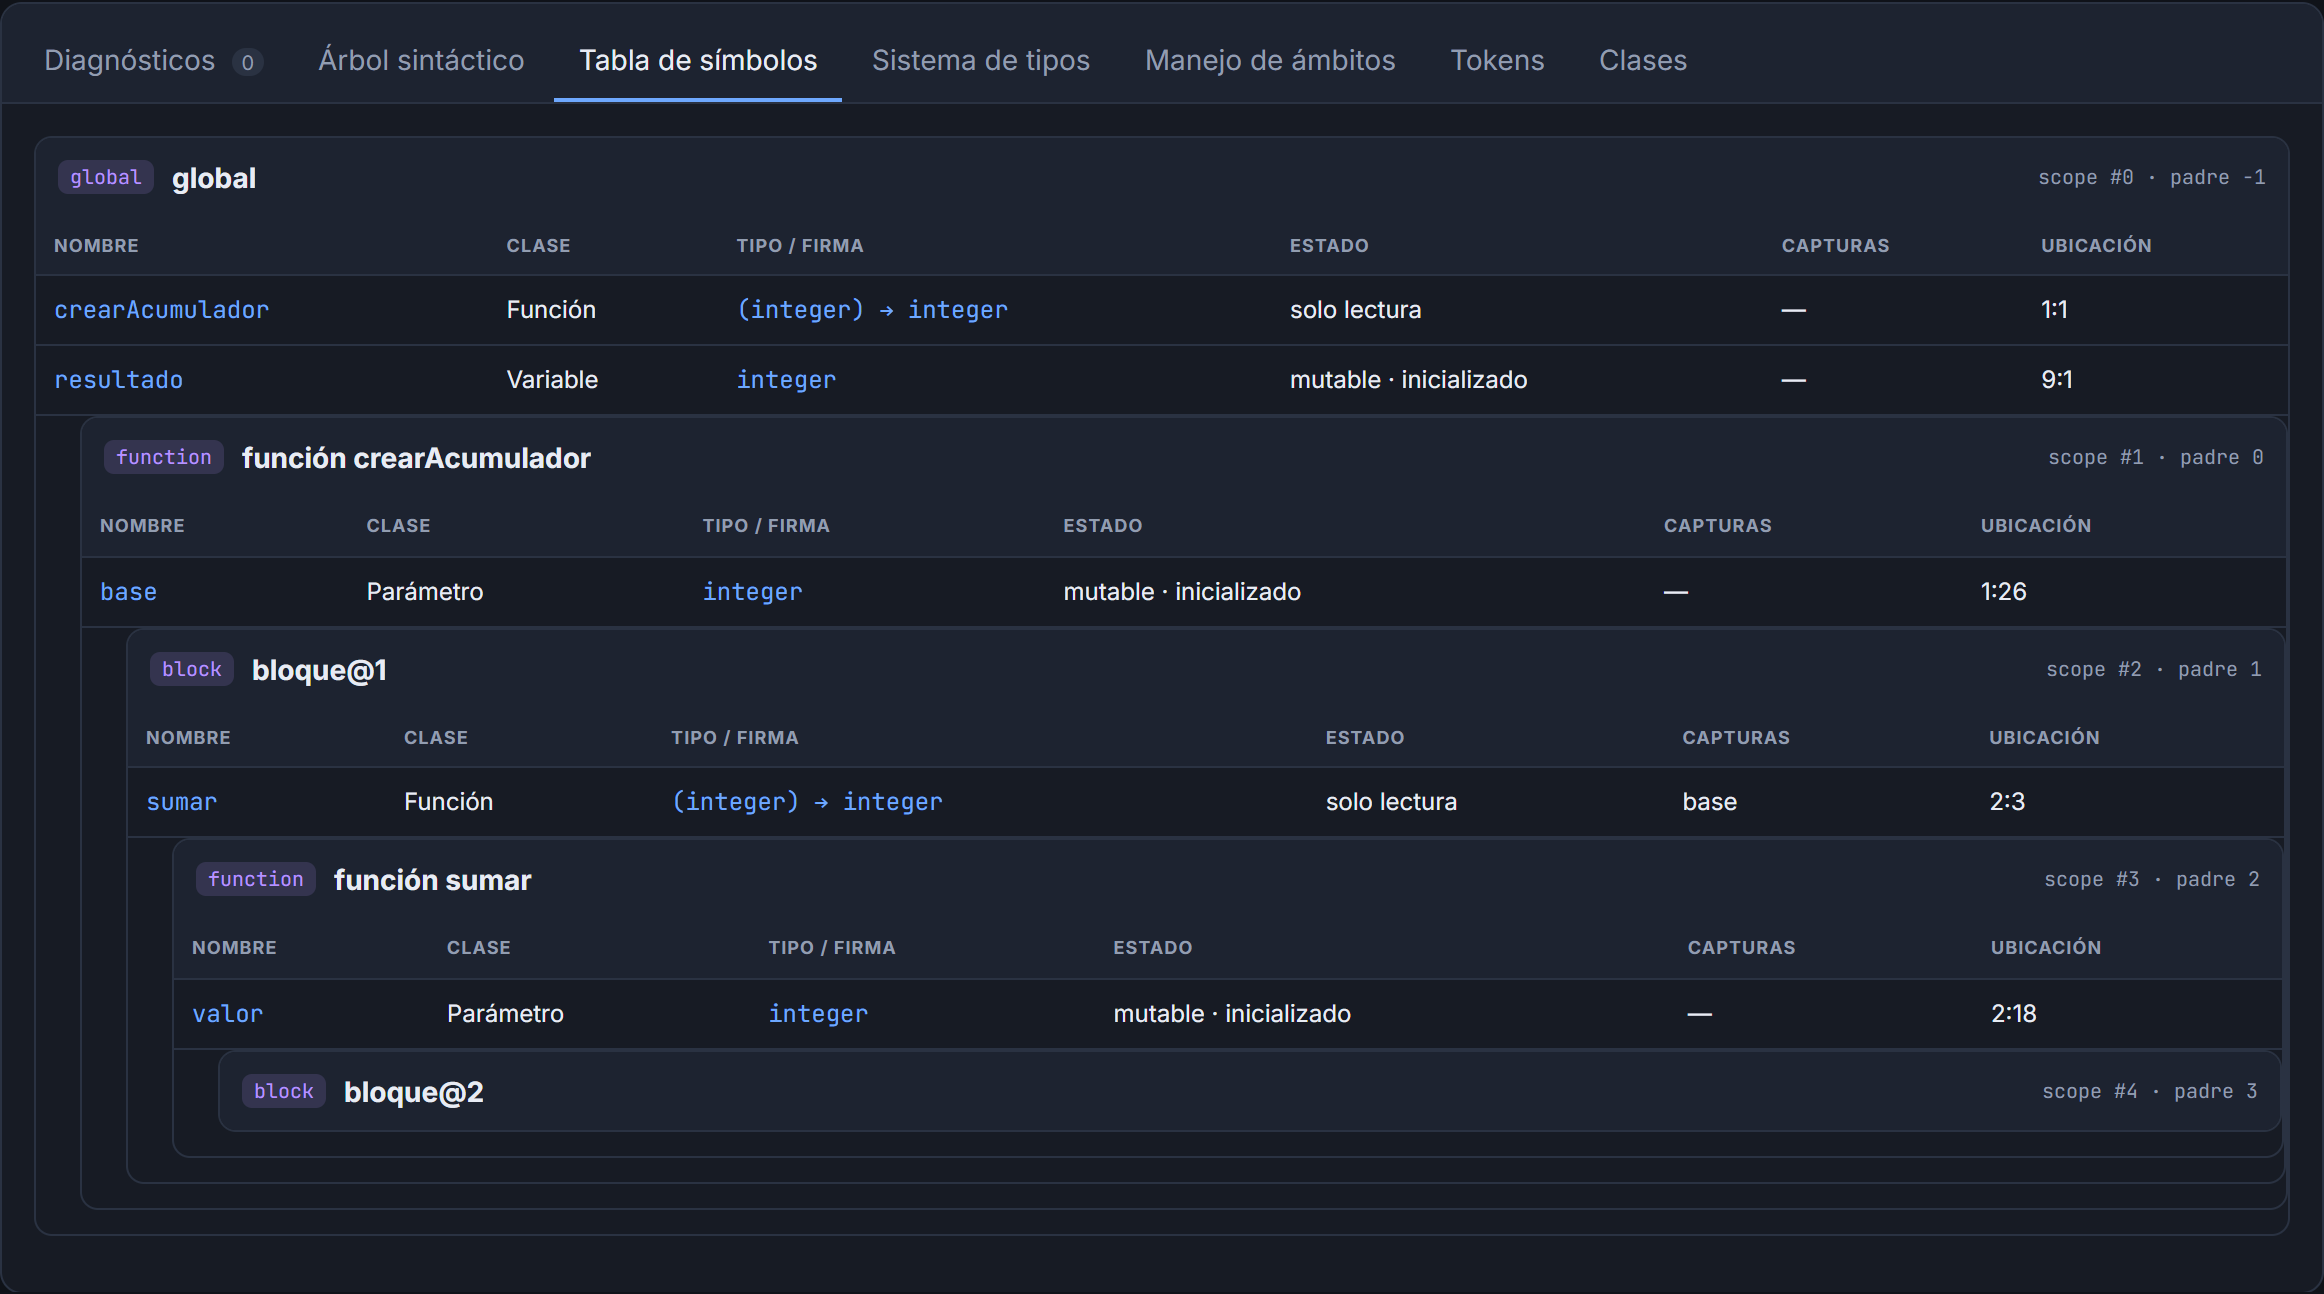
\includegraphics[width=\textwidth]{img/closures-simbolos.png}
\caption{Tabla de símbolos de \texttt{closures.cps}. La función anidada
\texttt{sumar} registra la captura del parámetro \texttt{base}.}
\end{figure}

% ------------------------------------------------------------------ 9 IDE
\section{El IDE}

El IDE es una aplicación web servida por Flask. Permite escribir, cargar,
guardar y descargar archivos \texttt{.cps}; analizar el programa con
\texttt{Ctrl/Cmd + Enter} o con el botón principal; navegar los diagnósticos
saltando a su ubicación; explorar el árbol sintáctico; consultar la tabla de
símbolos; revisar el sistema de tipos, los ámbitos, los tokens y las clases; y
ejecutar la batería de pruebas desde la propia interfaz.

\begin{figure}[H]
\centering
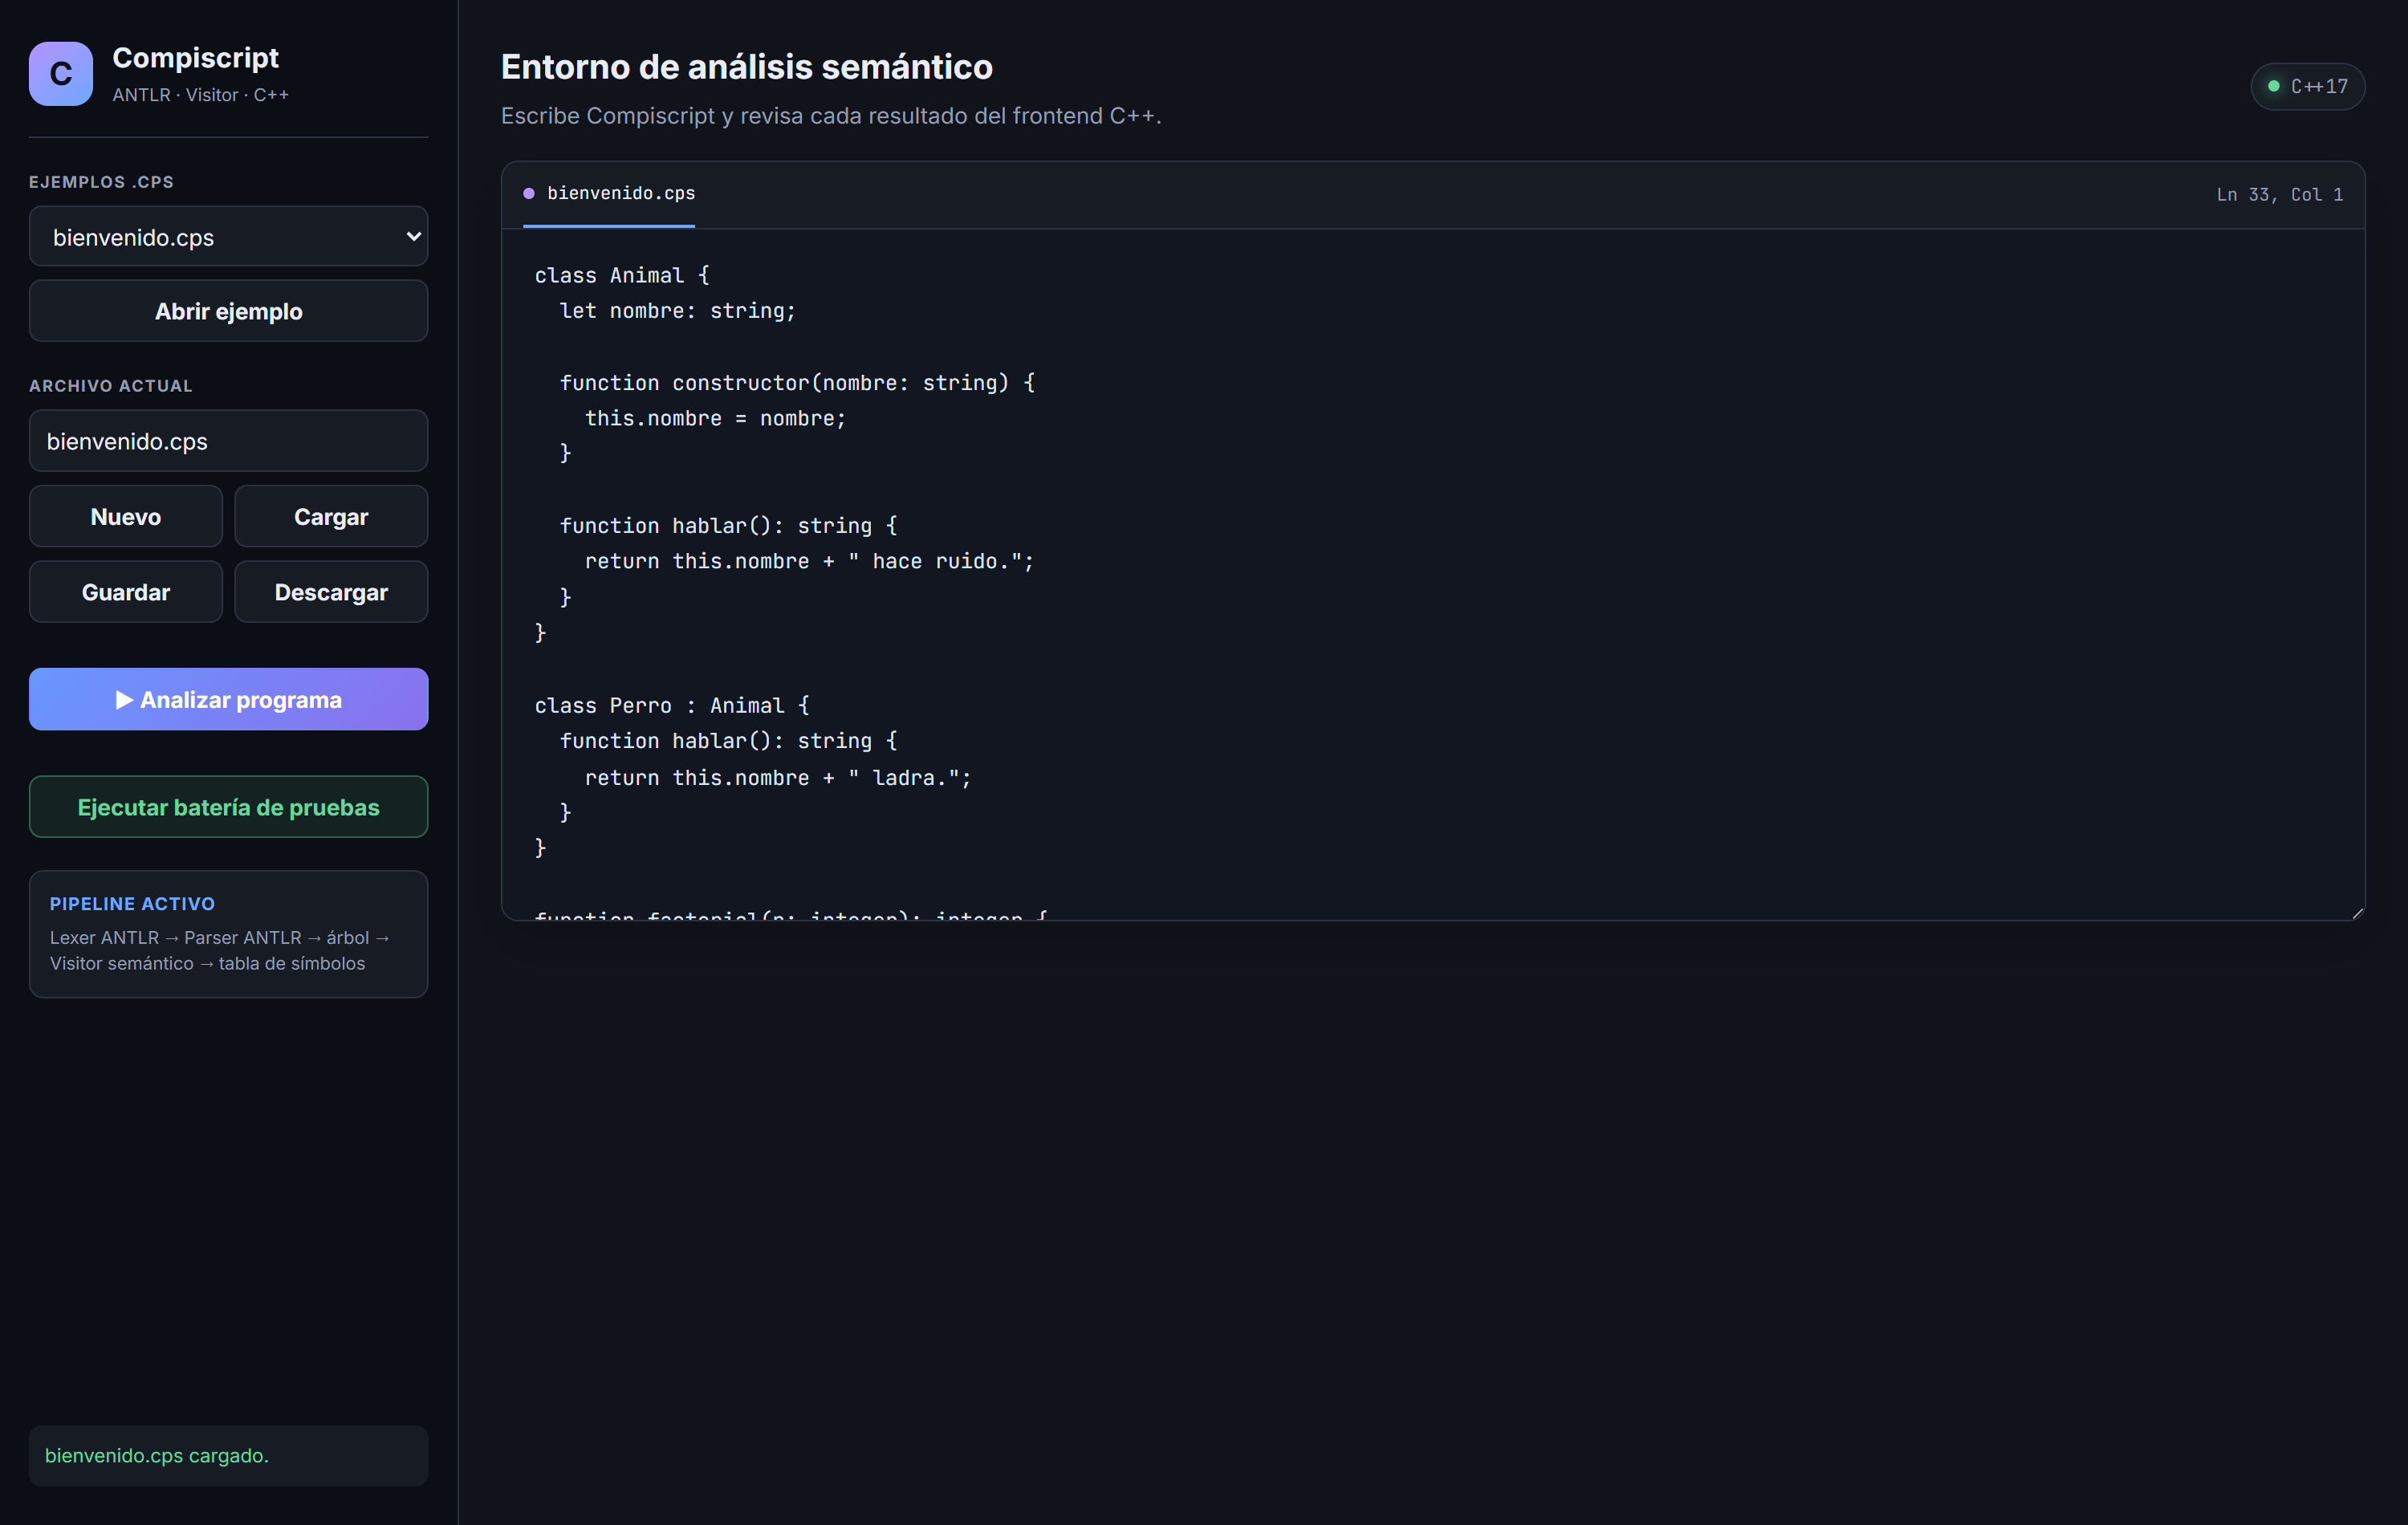
\includegraphics[width=\textwidth]{img/ide-inicial.png}
\caption{Estado inicial del IDE.}
\end{figure}

\begin{figure}[H]
\centering
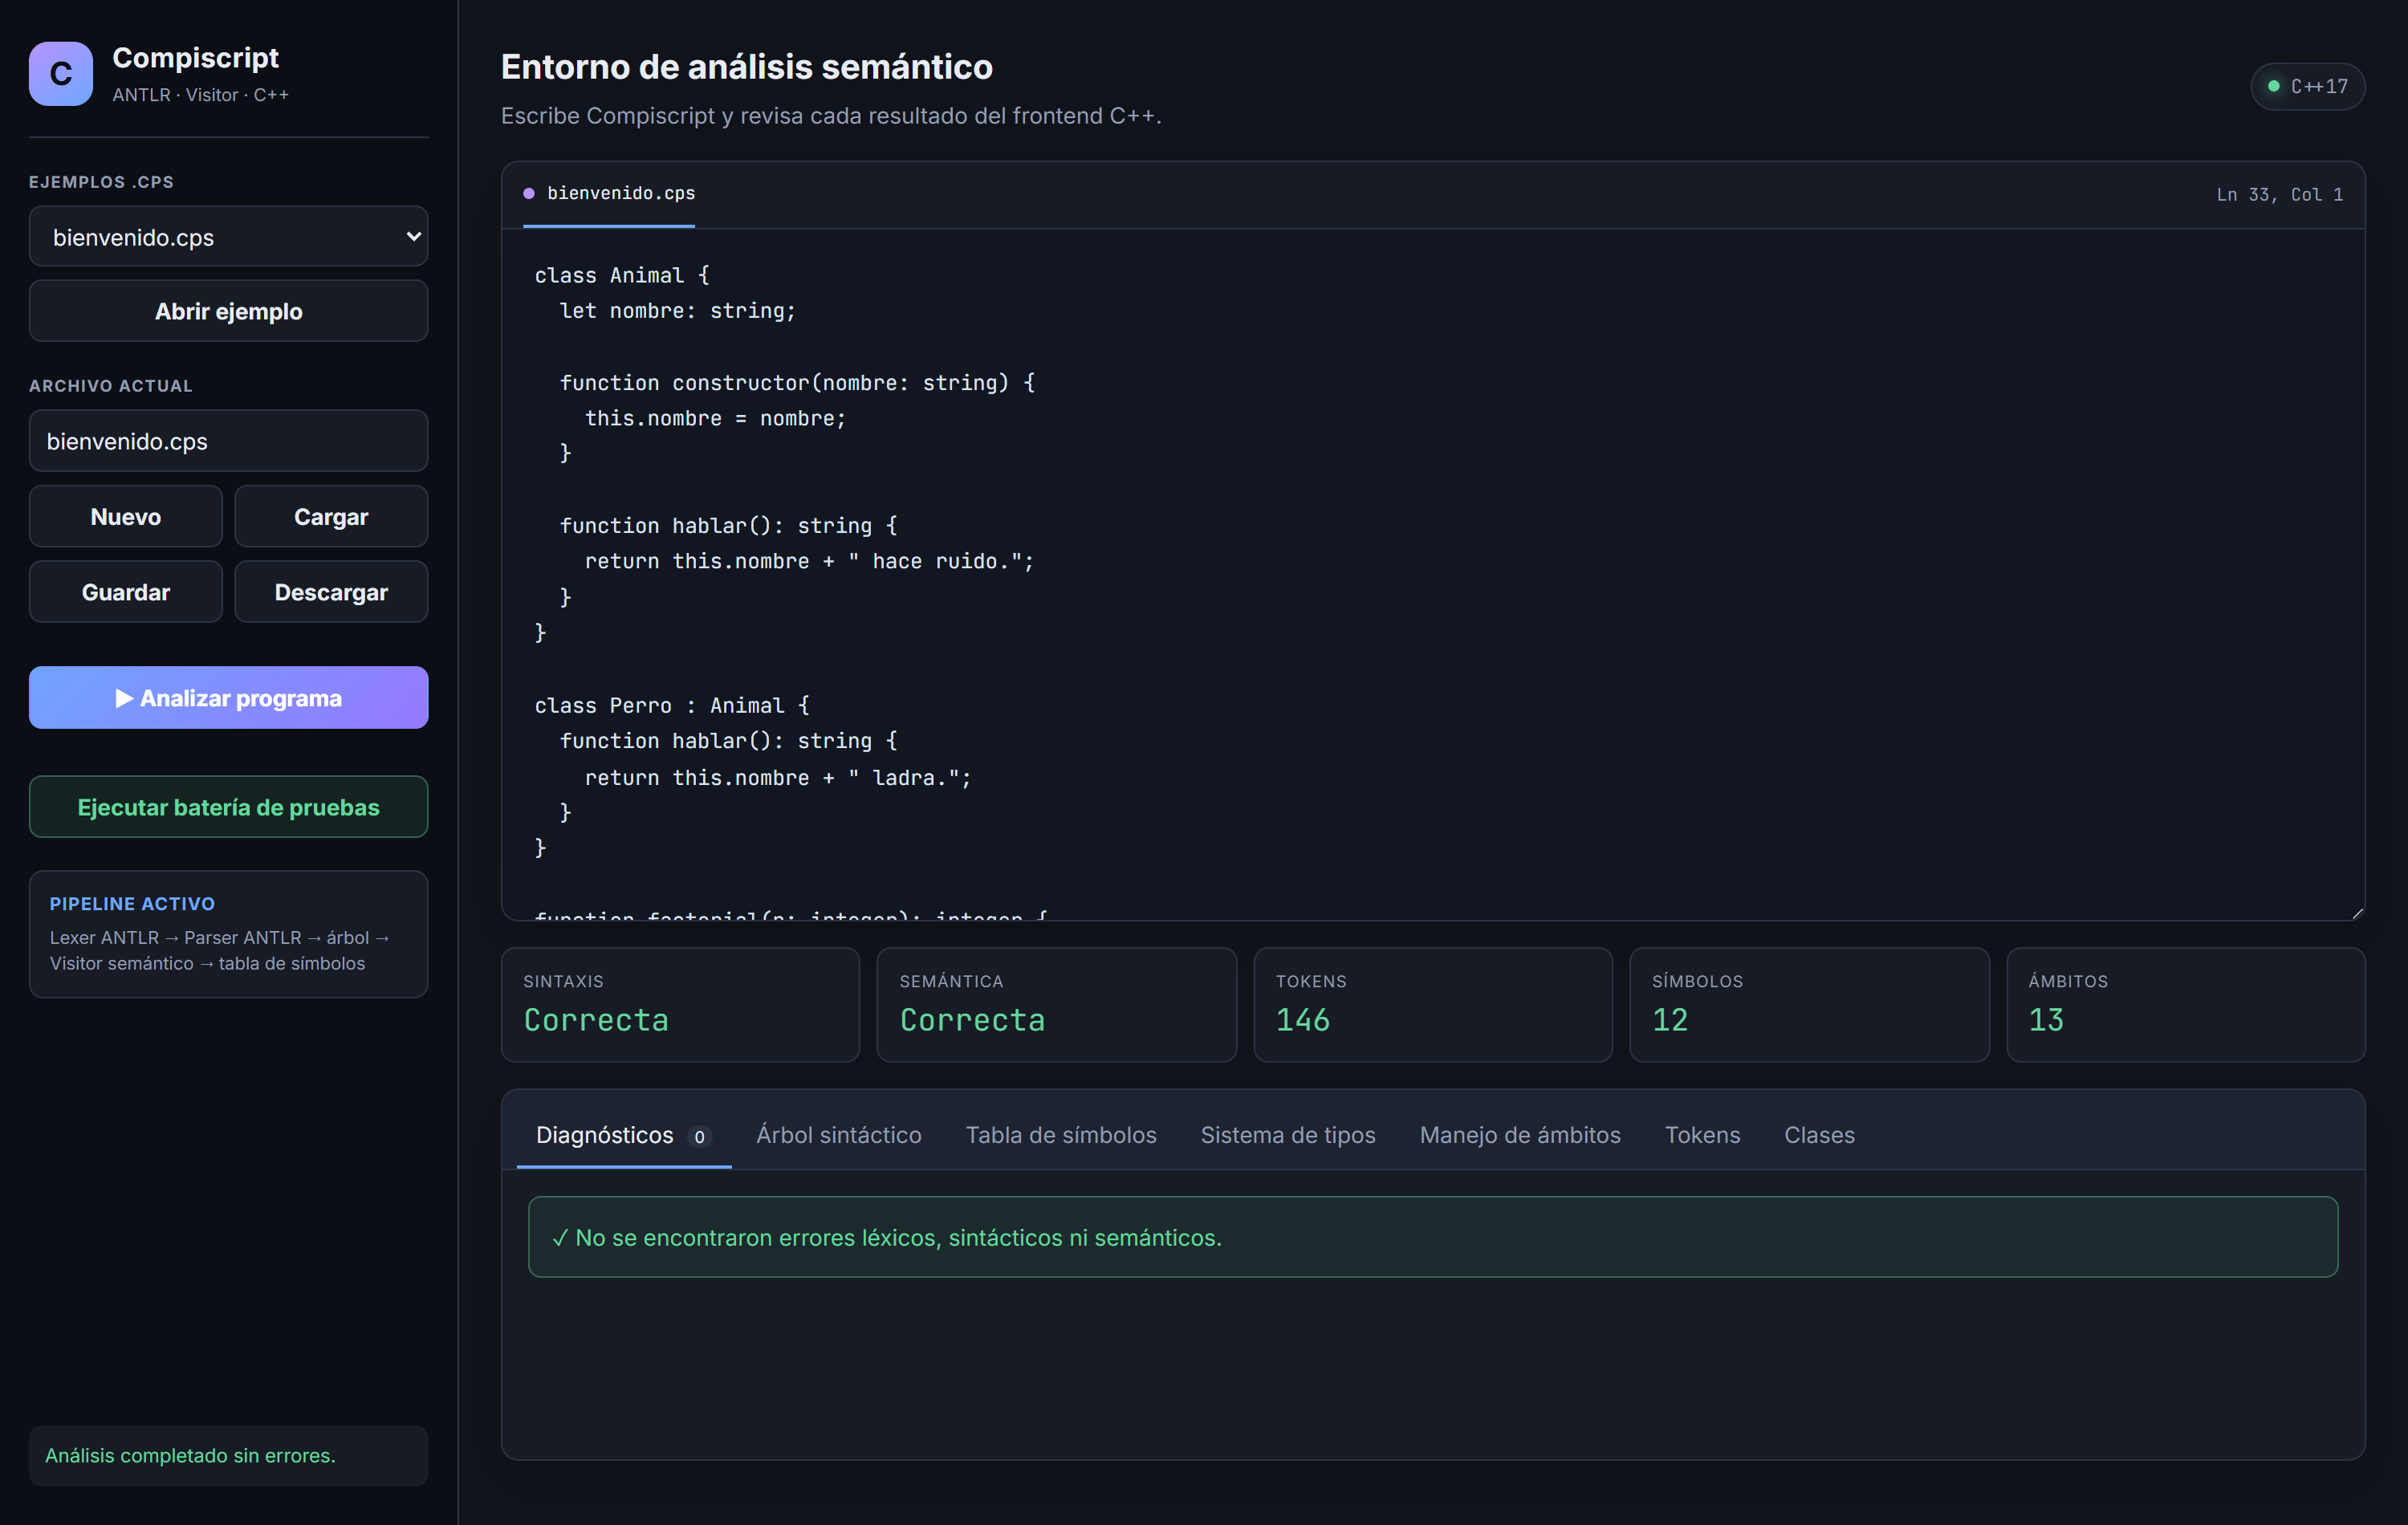
\includegraphics[width=\textwidth]{img/ide-general.png}
\caption{Análisis de \texttt{bienvenido.cps}: sintaxis y semántica correctas,
146 tokens, 12 símbolos y 13 ámbitos.}
\end{figure}

\subsection{Diagnósticos}

Cada diagnóstico muestra su código estable, la categoría a la que pertenece, el
mensaje y la ubicación \texttt{línea:columna}. Al hacer clic sobre uno, el
editor mueve el cursor a esa posición.

\begin{figure}[H]
\centering
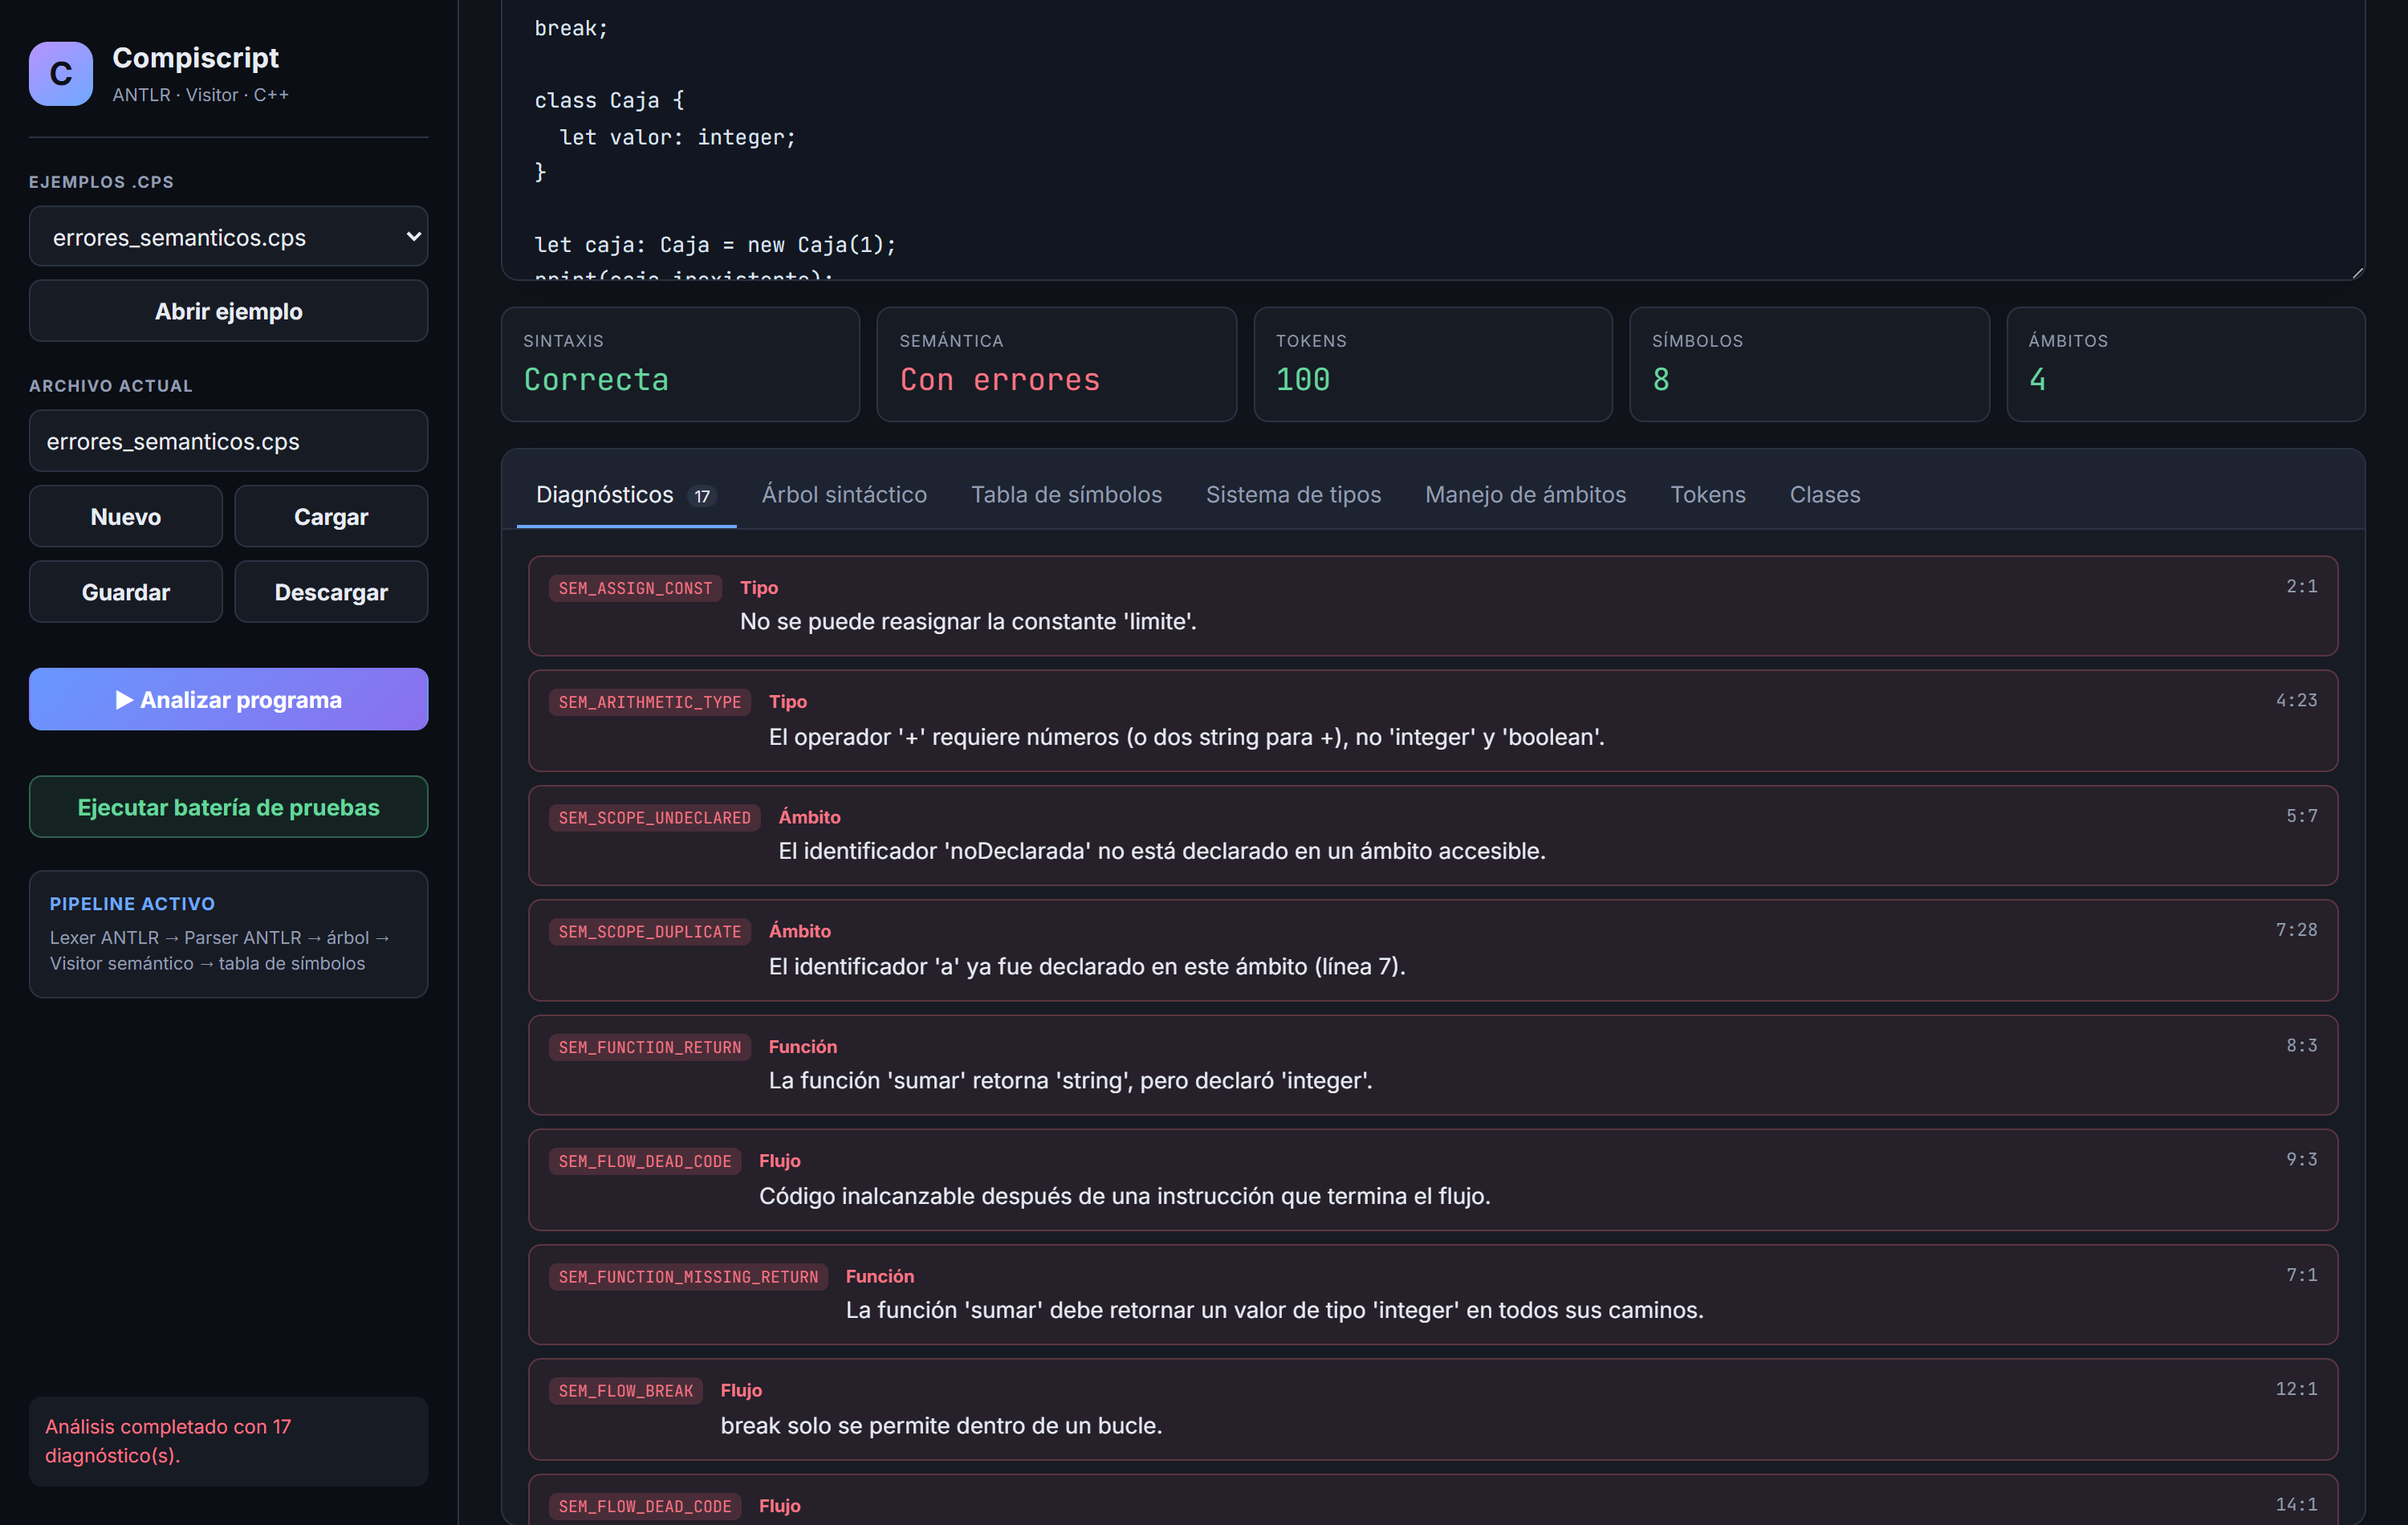
\includegraphics[width=\textwidth]{img/ide-errores.png}
\caption{Análisis de \texttt{errores\_semanticos.cps}: la sintaxis es correcta y
la semántica reporta 17 errores.}
\end{figure}

\begin{figure}[H]
\centering
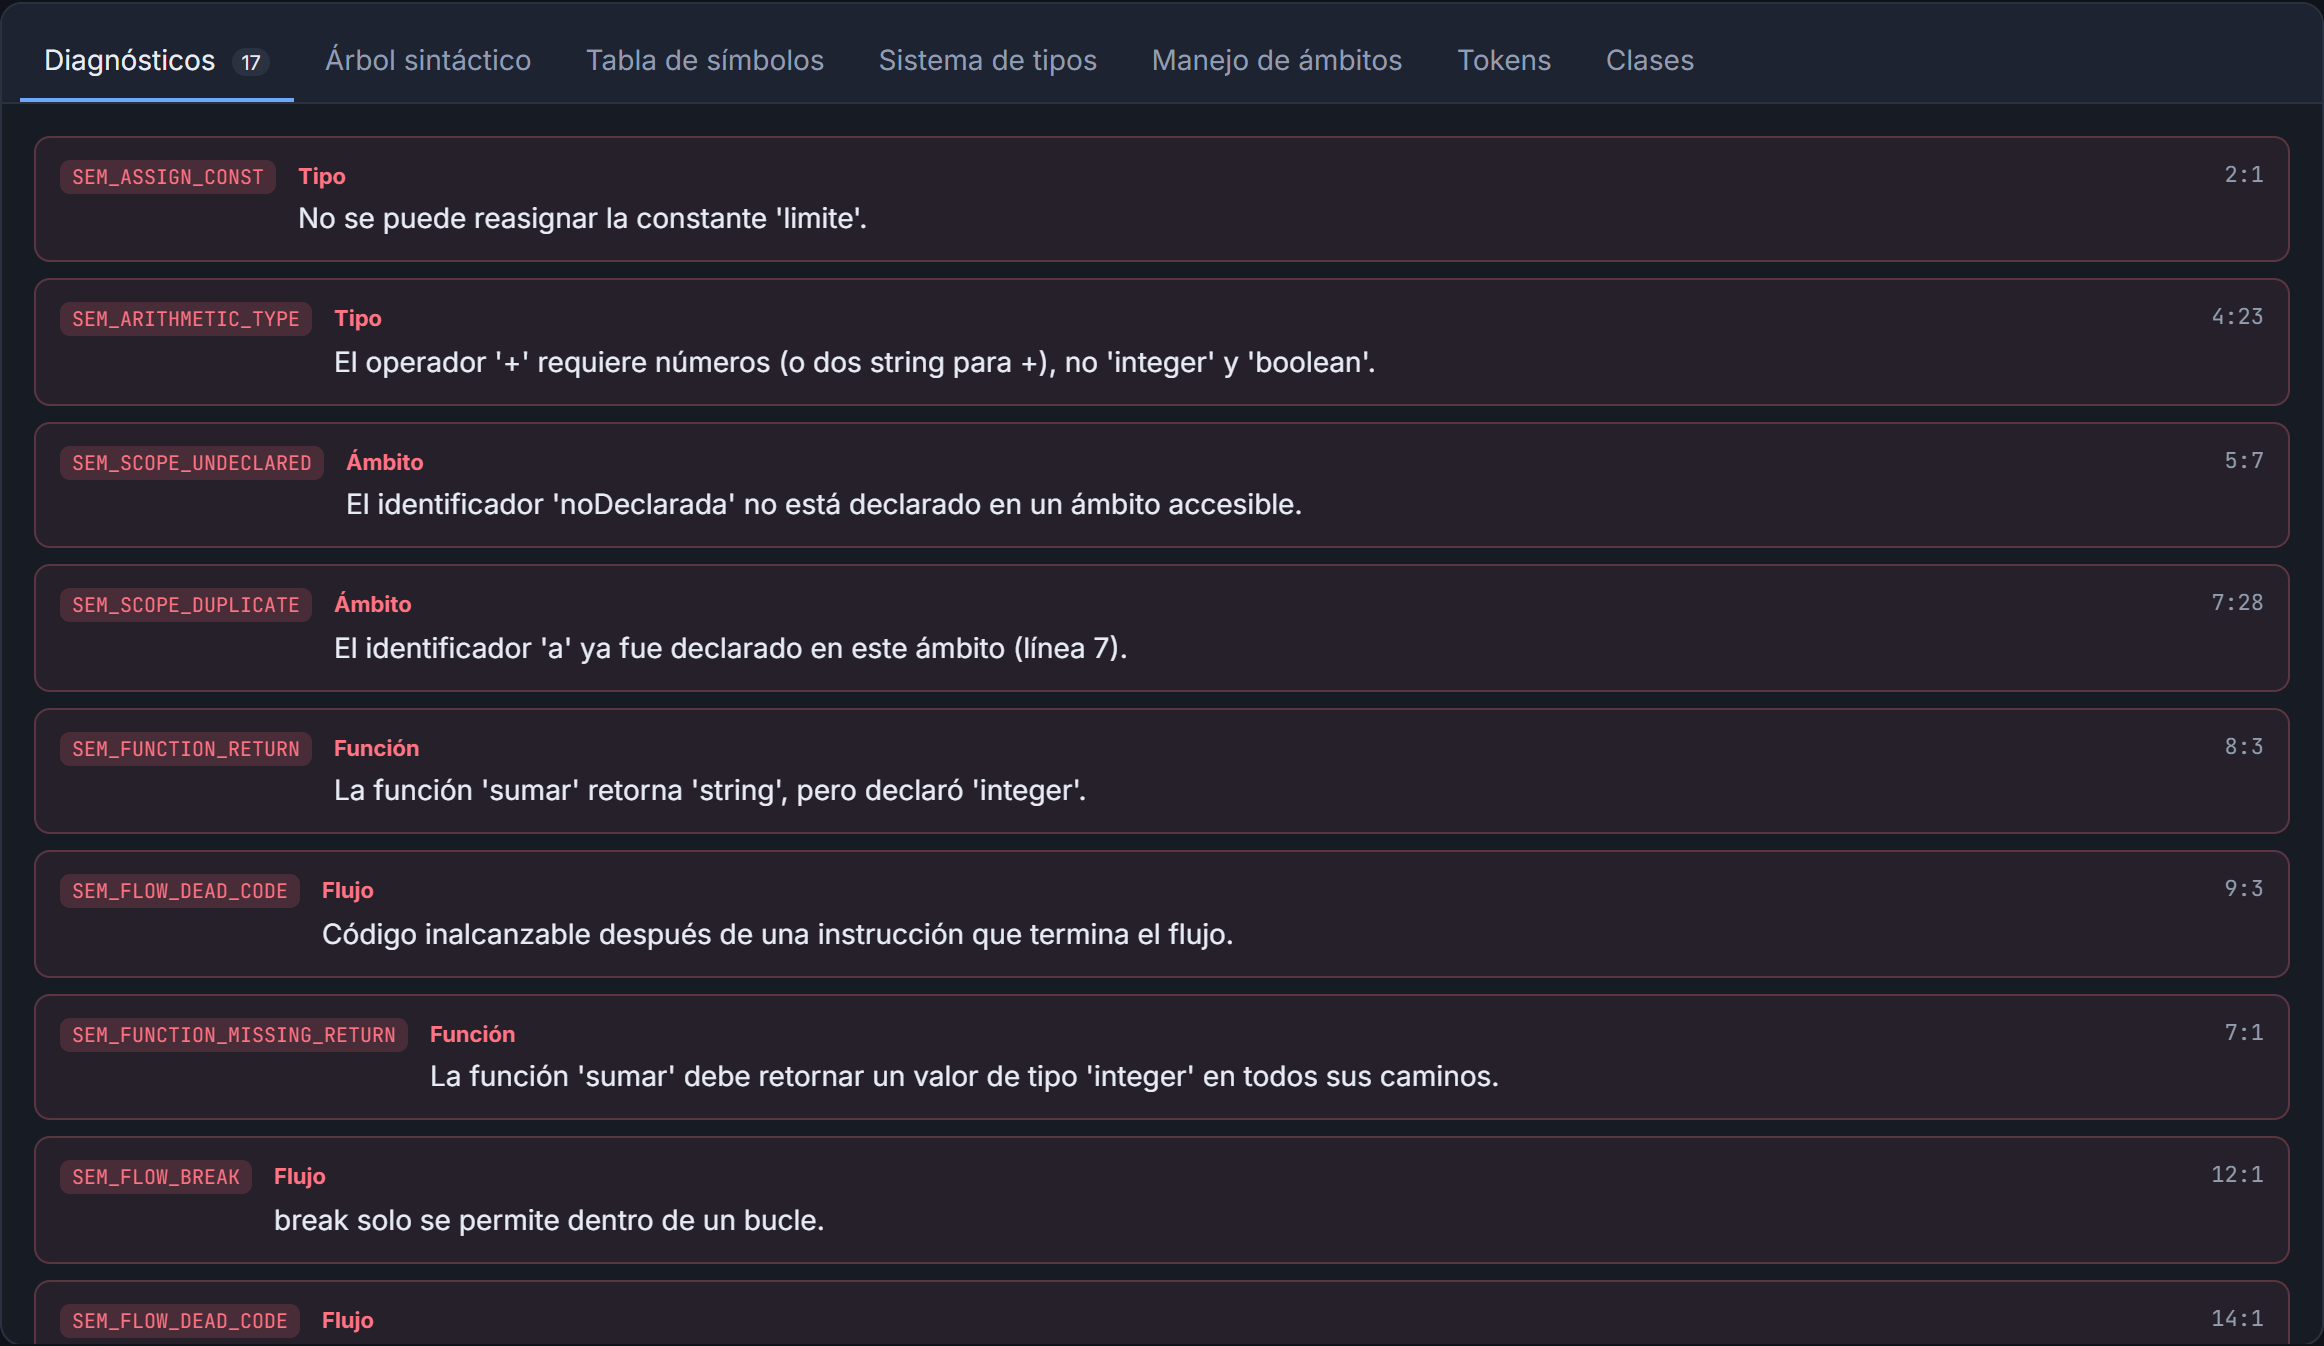
\includegraphics[width=\textwidth]{img/diagnosticos.png}
\caption{Panel de diagnósticos con las siete familias de reglas representadas.}
\end{figure}

\subsection{Árbol sintáctico}

El árbol es la serialización del parse tree que produce ANTLR. Cada nodo indica
la regla o el token, su posición y el número de hijos; se puede expandir,
contraer y ampliar.

\begin{figure}[H]
\centering
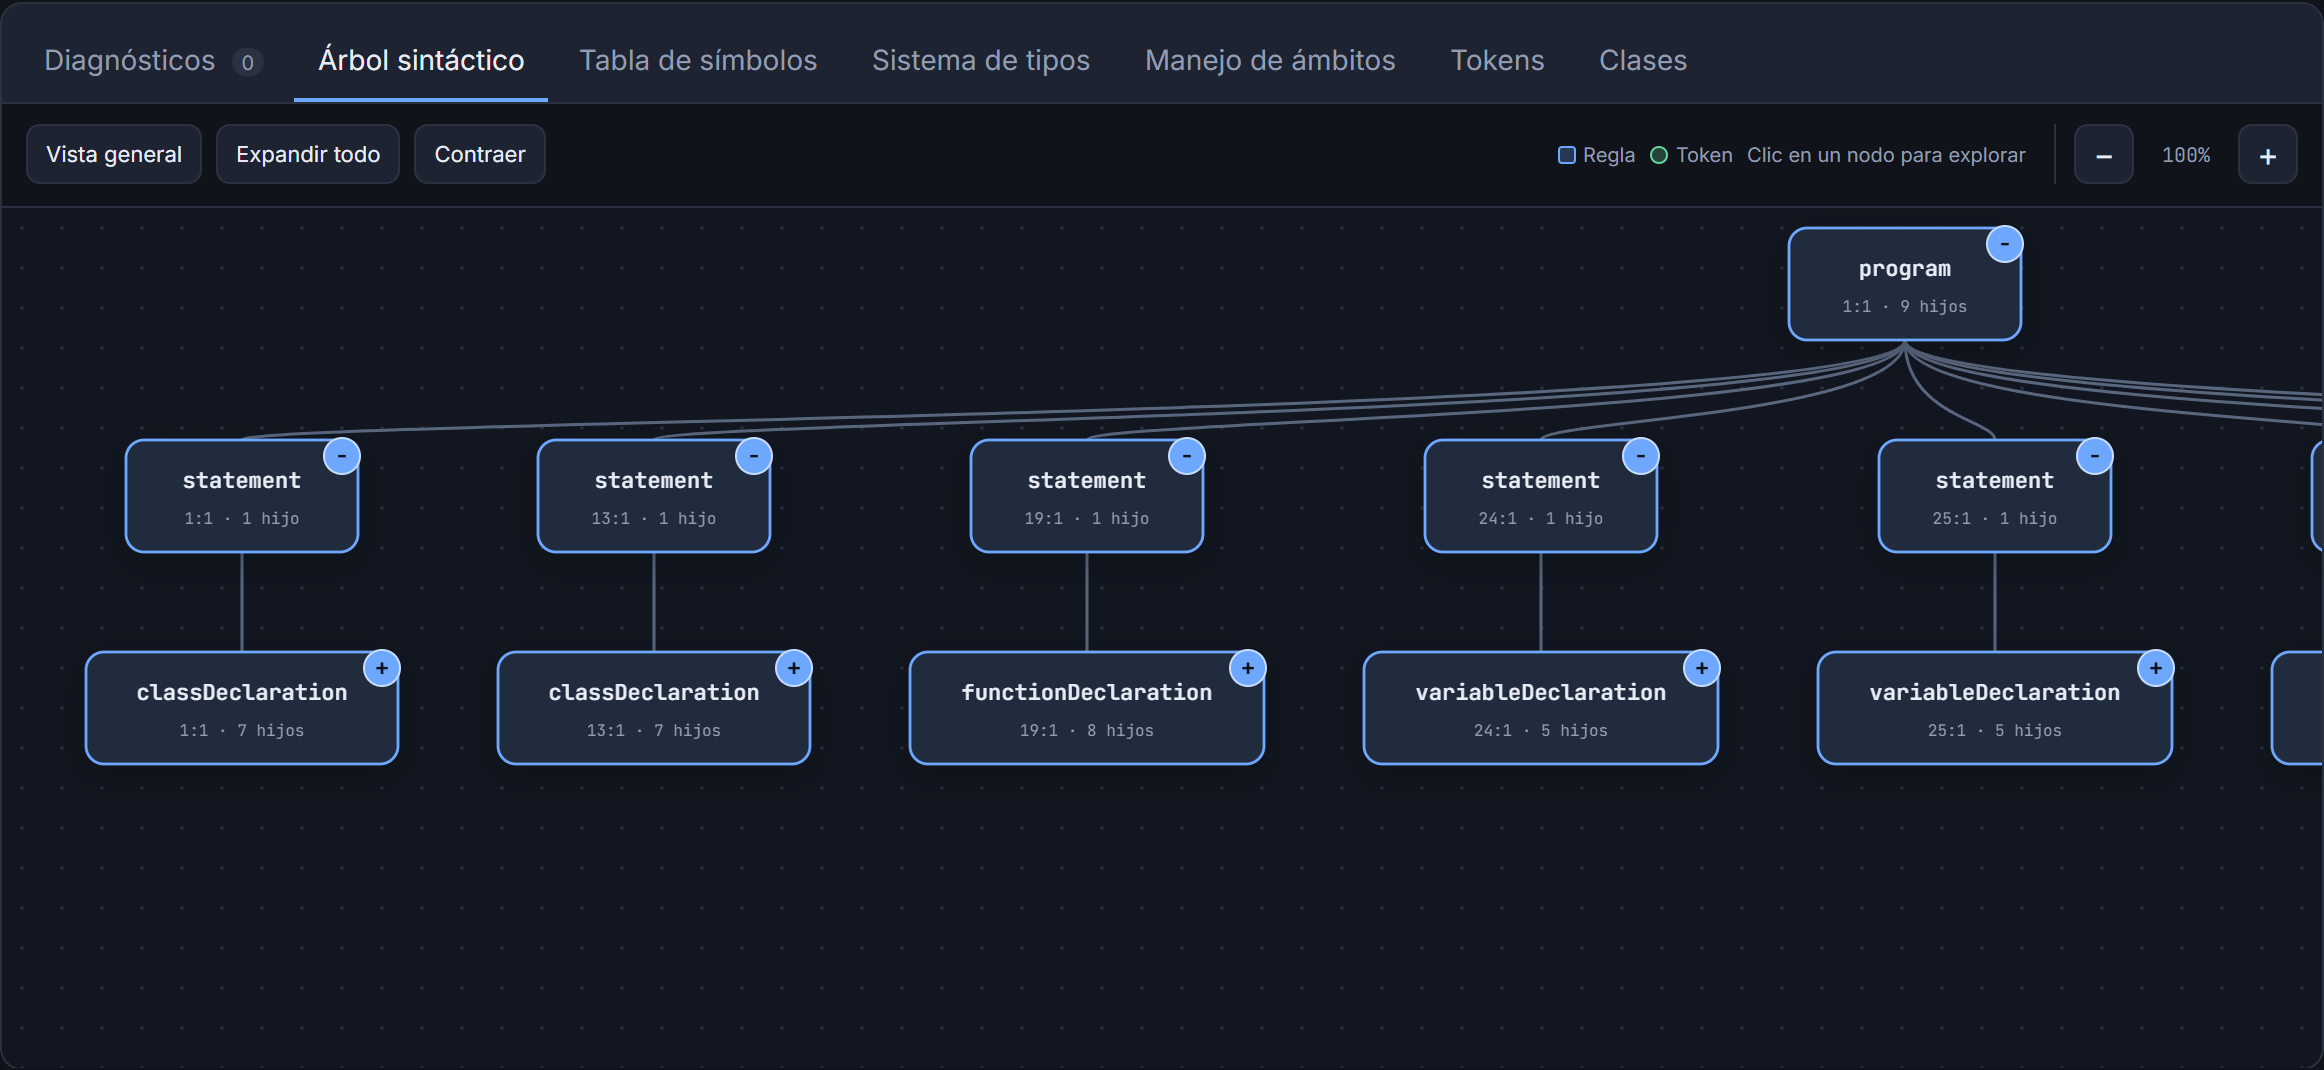
\includegraphics[width=\textwidth]{img/arbol.png}
\caption{Representación visual del árbol sintáctico.}
\end{figure}

\subsection{Tabla de símbolos y ámbitos}

\begin{figure}[H]
\centering
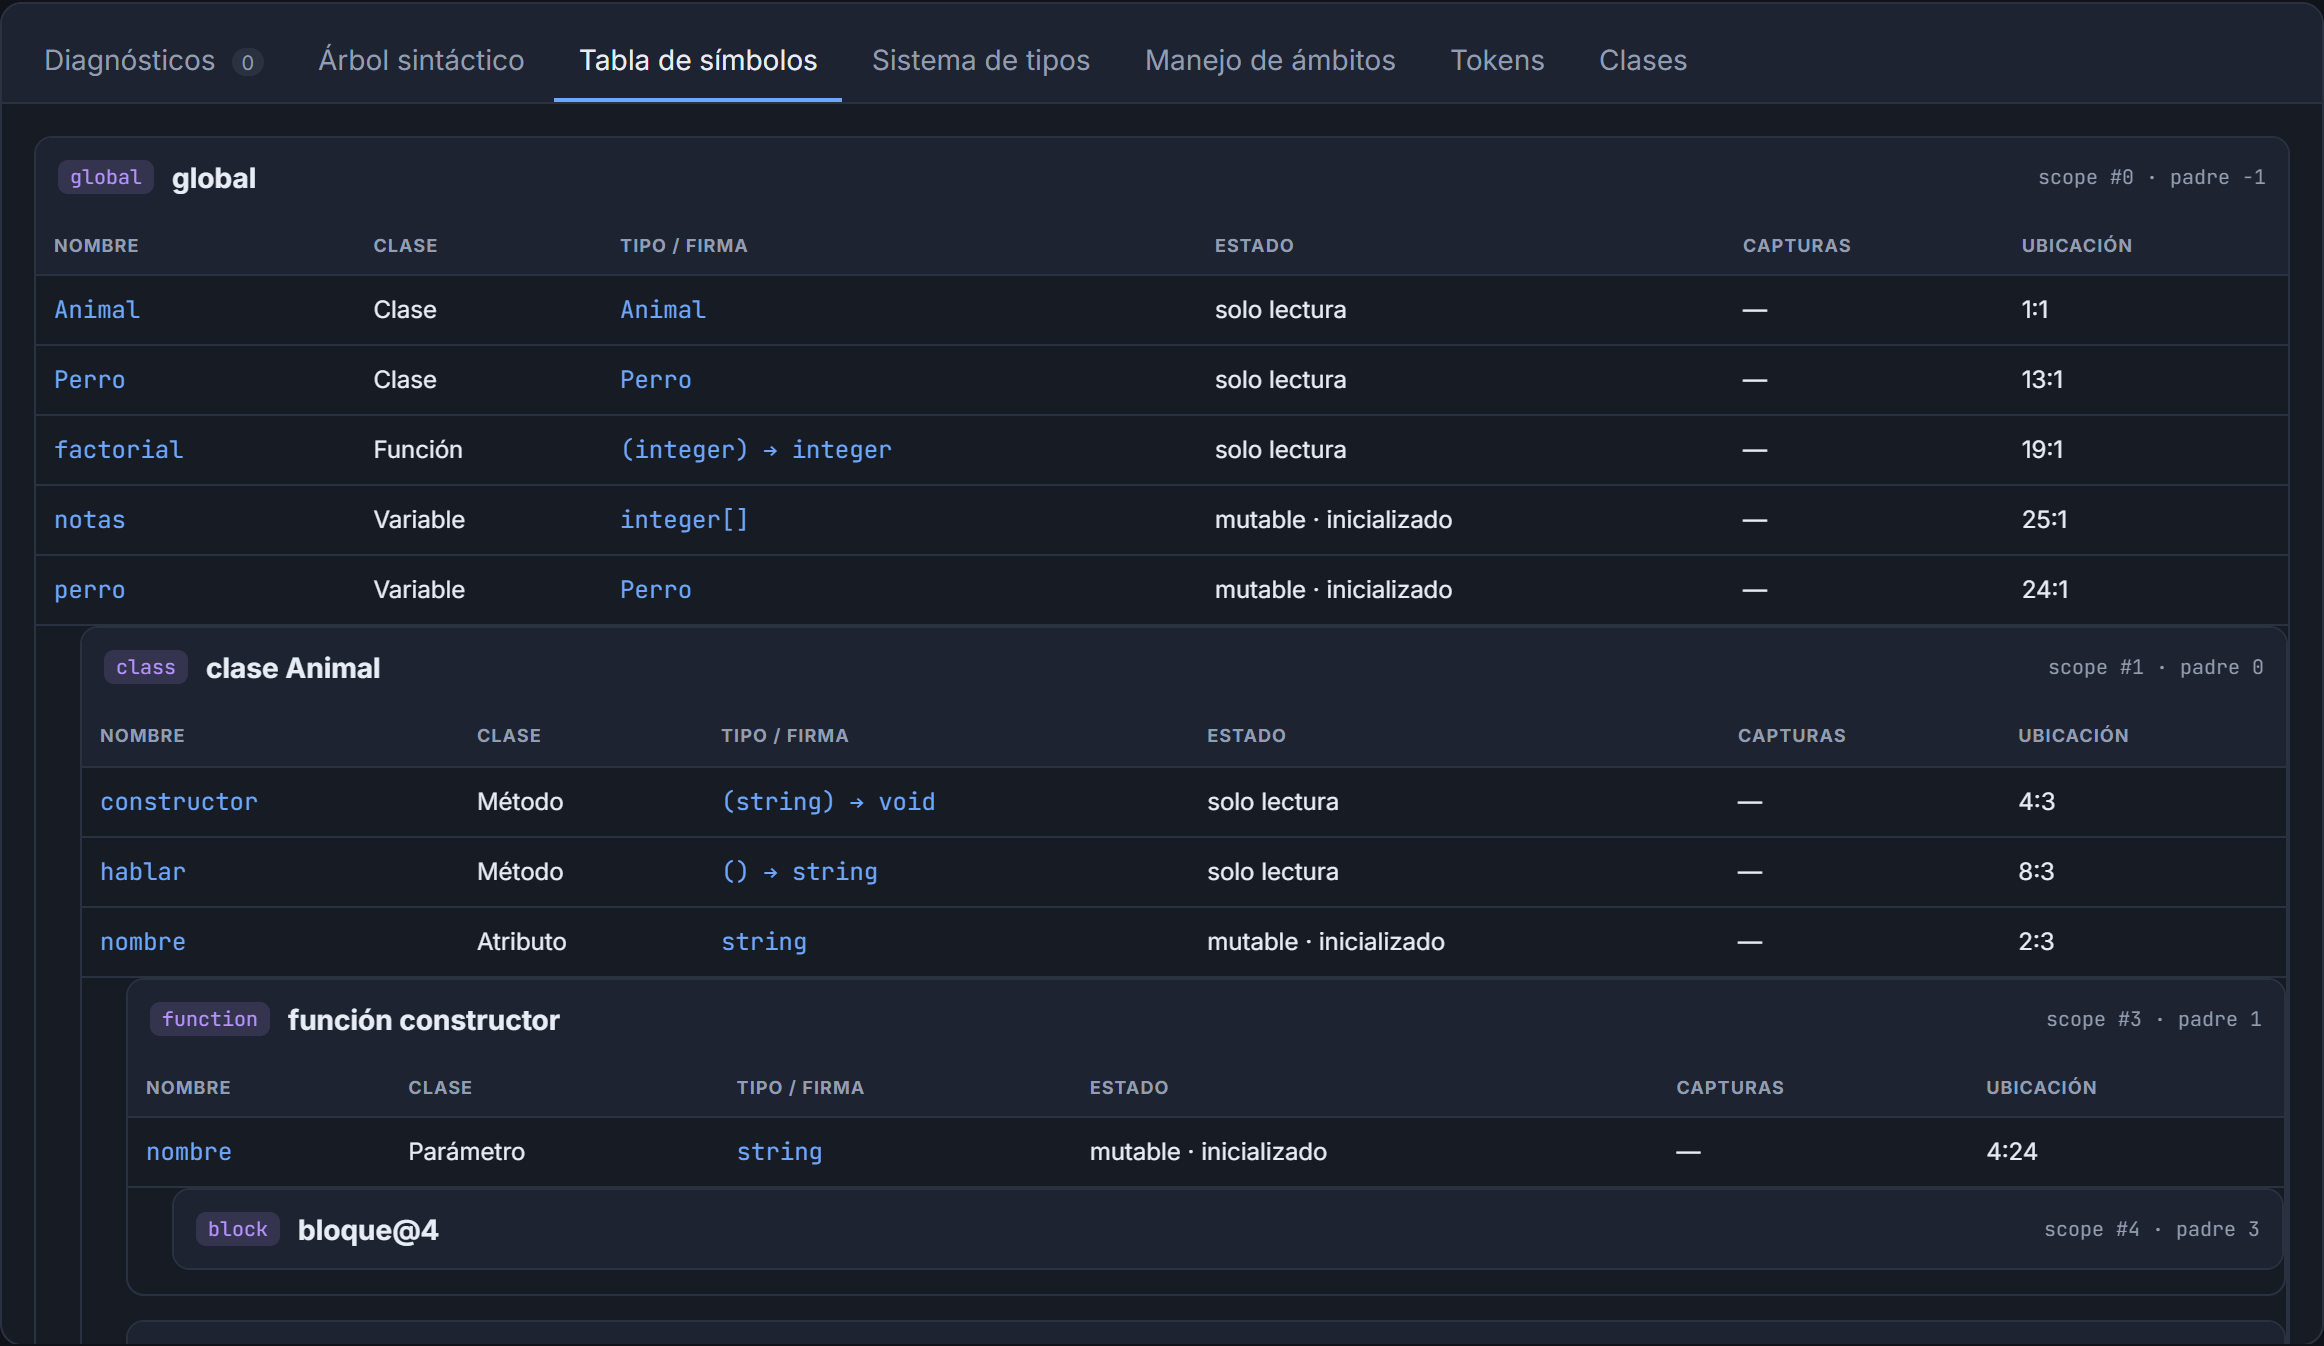
\includegraphics[width=\textwidth]{img/simbolos.png}
\caption{Tabla de símbolos jerárquica: cada entorno lista sus símbolos con
clase, tipo o firma, estado, capturas y ubicación.}
\end{figure}

\begin{figure}[H]
\centering
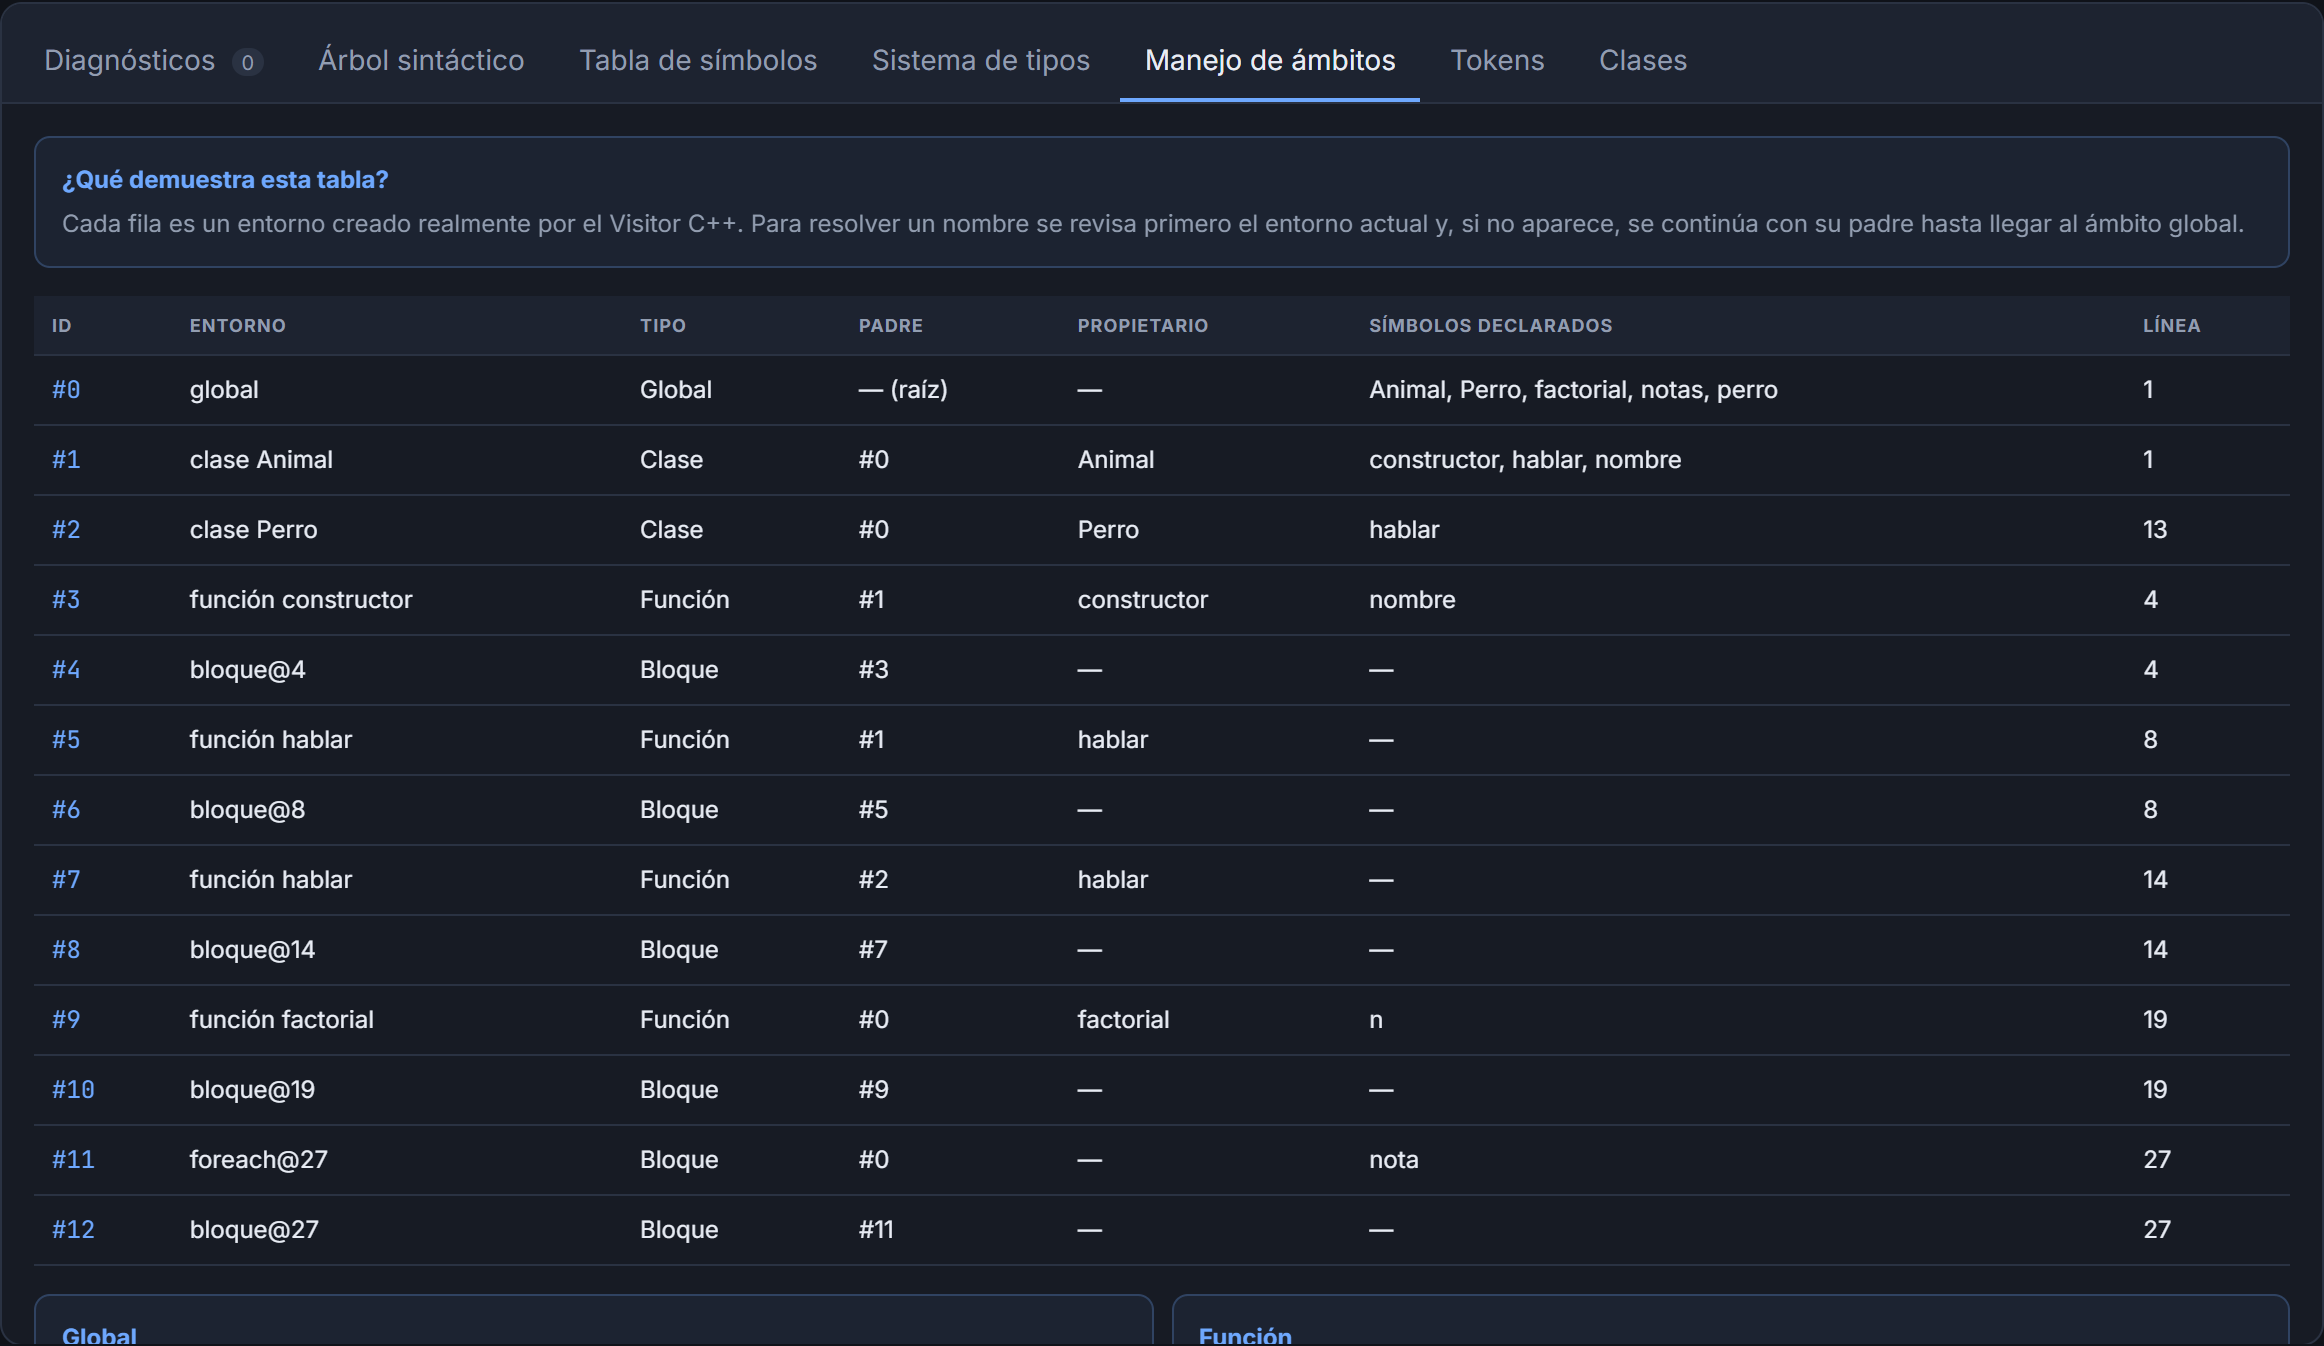
\includegraphics[width=\textwidth]{img/ambitos.png}
\caption{Vista tabular de ámbitos: identificador, clase de entorno, padre,
propietario y símbolos declarados.}
\end{figure}

\subsection{Sistema de tipos, tokens y clases}

\begin{figure}[H]
\centering
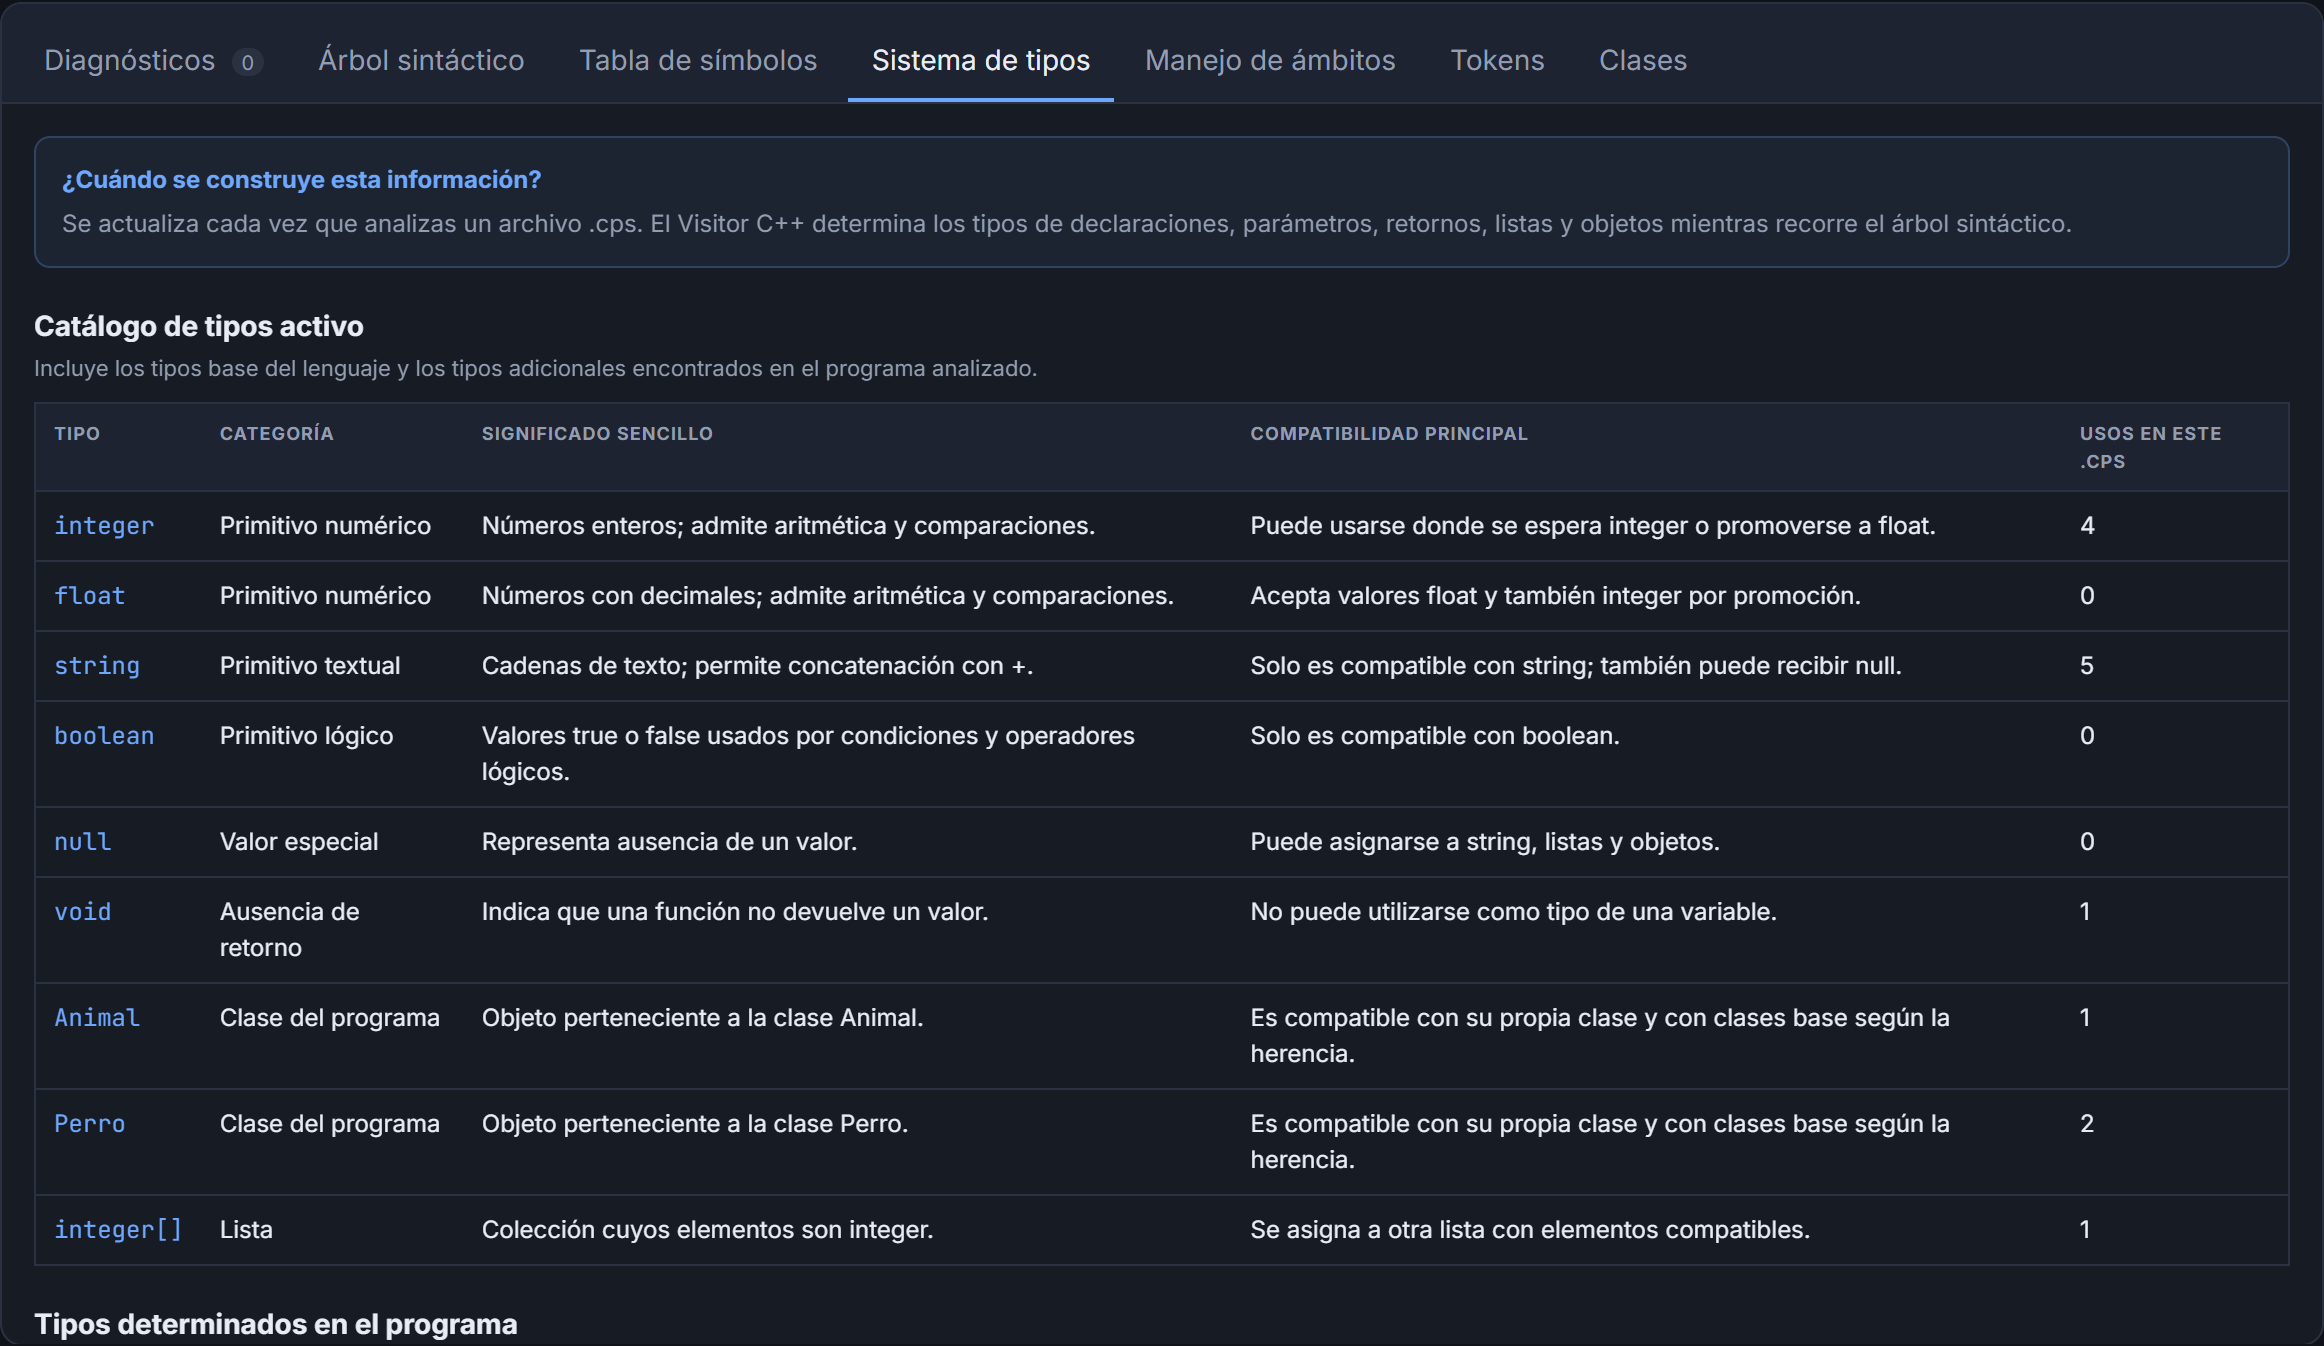
\includegraphics[width=\textwidth]{img/tipos.png}
\caption{Sistema de tipos activo y tipos determinados en el programa.}
\end{figure}

\begin{figure}[H]
\centering
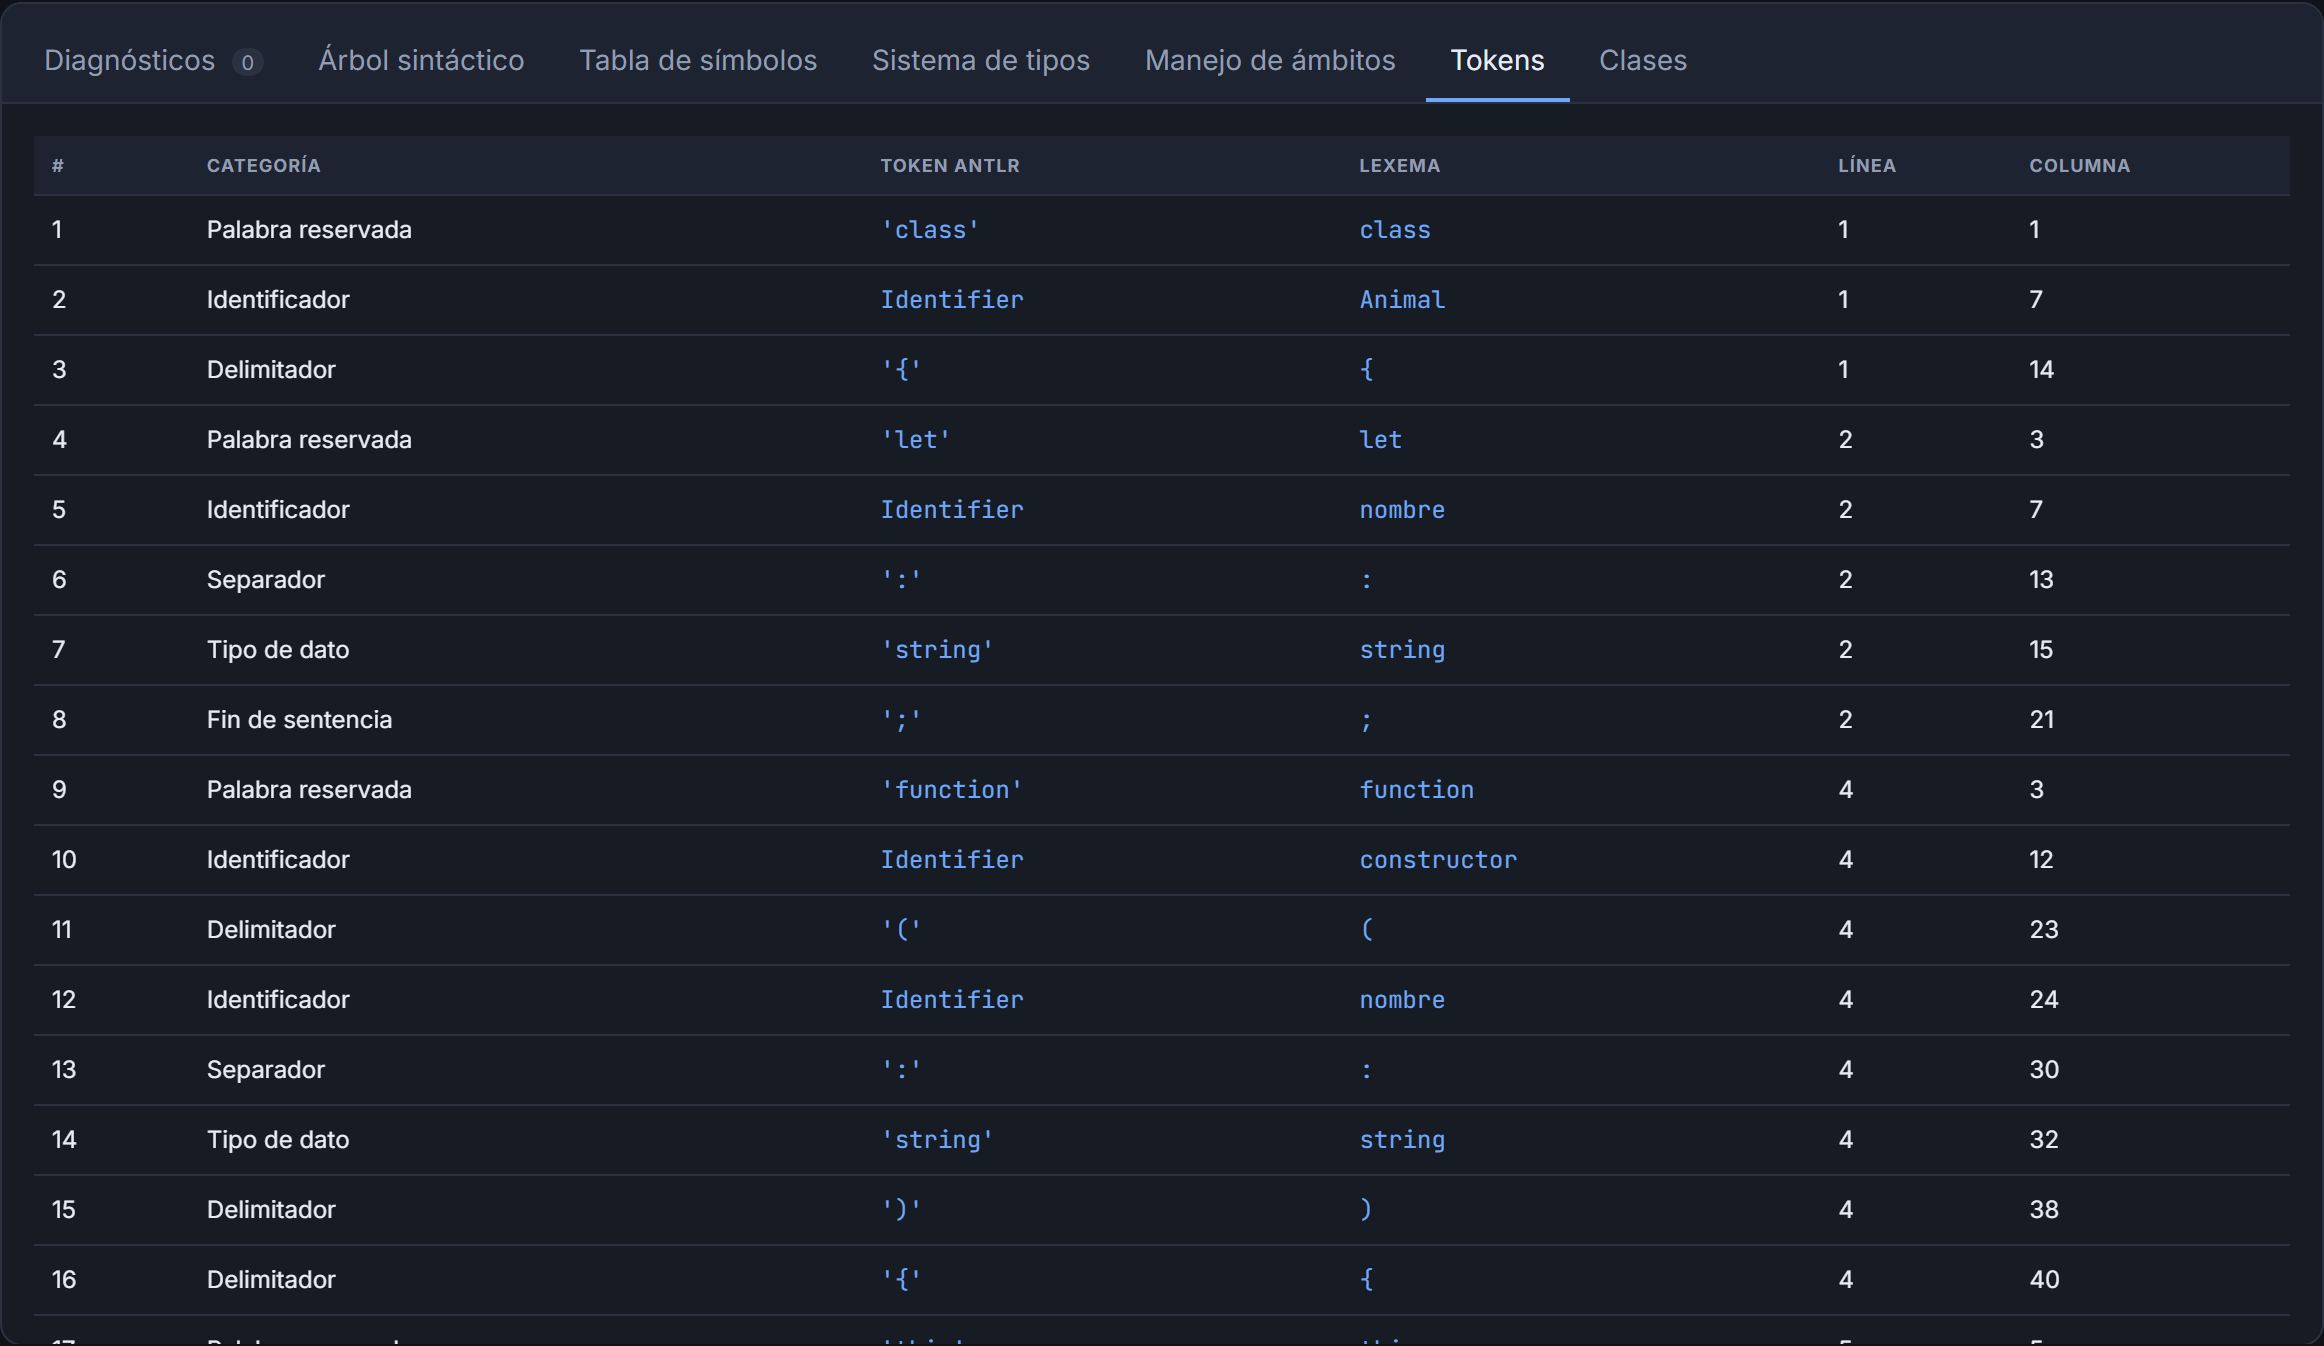
\includegraphics[width=\textwidth]{img/tokens.png}
\caption{Tokens producidos por el lexer de ANTLR, con categoría, lexema y
posición.}
\end{figure}

\begin{figure}[H]
\centering
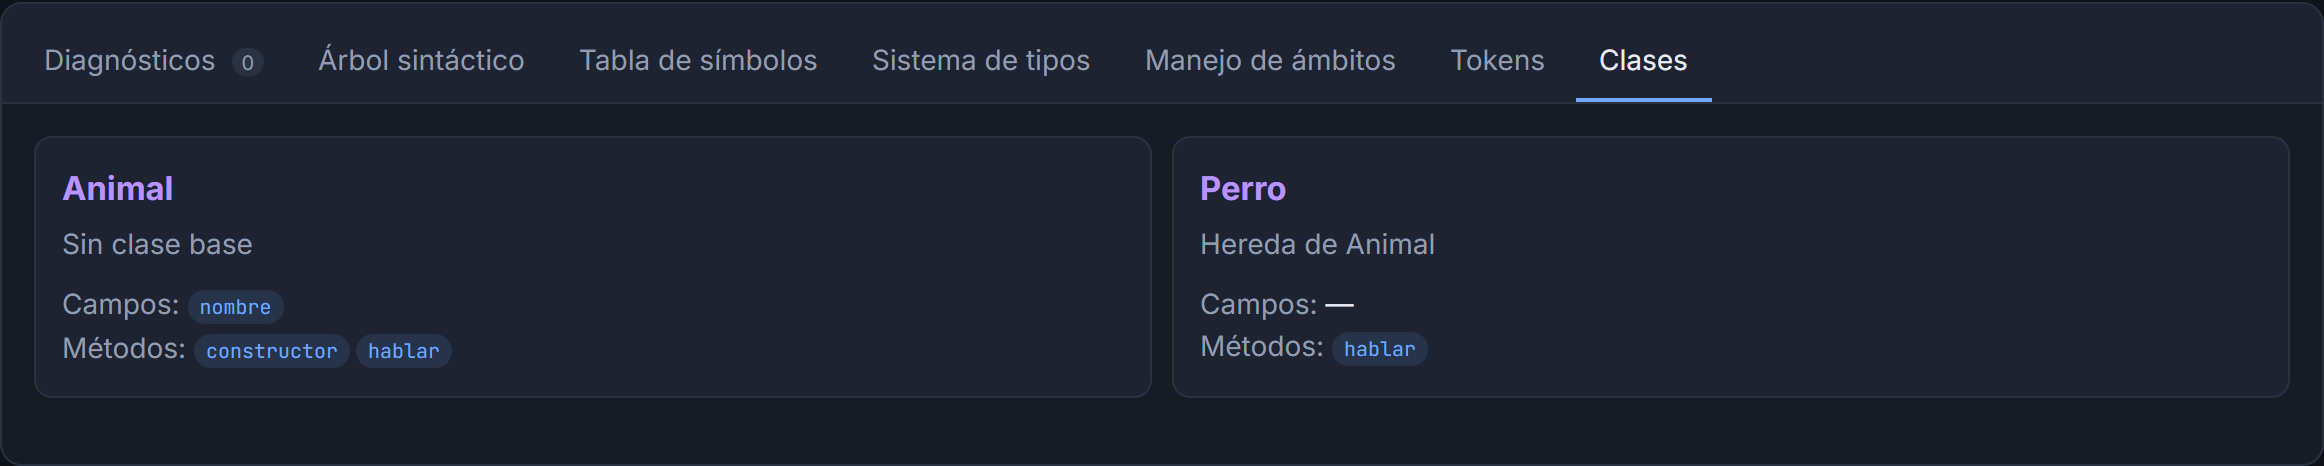
\includegraphics[width=\textwidth]{img/clases.png}
\caption{Clases declaradas con su clase base, campos y métodos.}
\end{figure}

% ----------------------------------------------------------- 10 PRUEBAS
\section{Batería de pruebas}

La batería está en \texttt{backend/tests/compiscript\_tests.cpp} y contiene
\textbf{95 escenarios}: 41 programas válidos y 54 errores esperados. No depende
de ningún framework externo; enlaza directamente contra
\texttt{compiscript\_core}, de modo que prueba el mismo servicio que usan el CLI
y el IDE.

El criterio de aprobación de un caso negativo es estricto: no basta con que el
programa falle, sino que debe fallar \textbf{con el código de diagnóstico
correcto}. Un programa que fuese rechazado por la razón equivocada se contaría
como fallo.

\begin{table}[H]
\centering
\small
\begin{tabular}{@{}lrr@{}}
\toprule
\textbf{Categoría} & \textbf{Aprobadas} & \textbf{Total} \\
\midrule
Proceso completo               & 4  & 4  \\
Sistema de tipos               & 20 & 20 \\
Manejo de ámbito               & 7  & 7  \\
Funciones y procedimientos     & 13 & 13 \\
Control de flujo               & 20 & 20 \\
Clases y objetos               & 13 & 13 \\
Listas y estructuras de datos  & 11 & 11 \\
Reglas generales               & 7  & 7  \\
\midrule
\textbf{Total}                 & \textbf{95} & \textbf{95} \\
\bottomrule
\end{tabular}
\caption{Resultado de la batería por categoría.}
\end{table}

\begin{figure}[H]
\centering
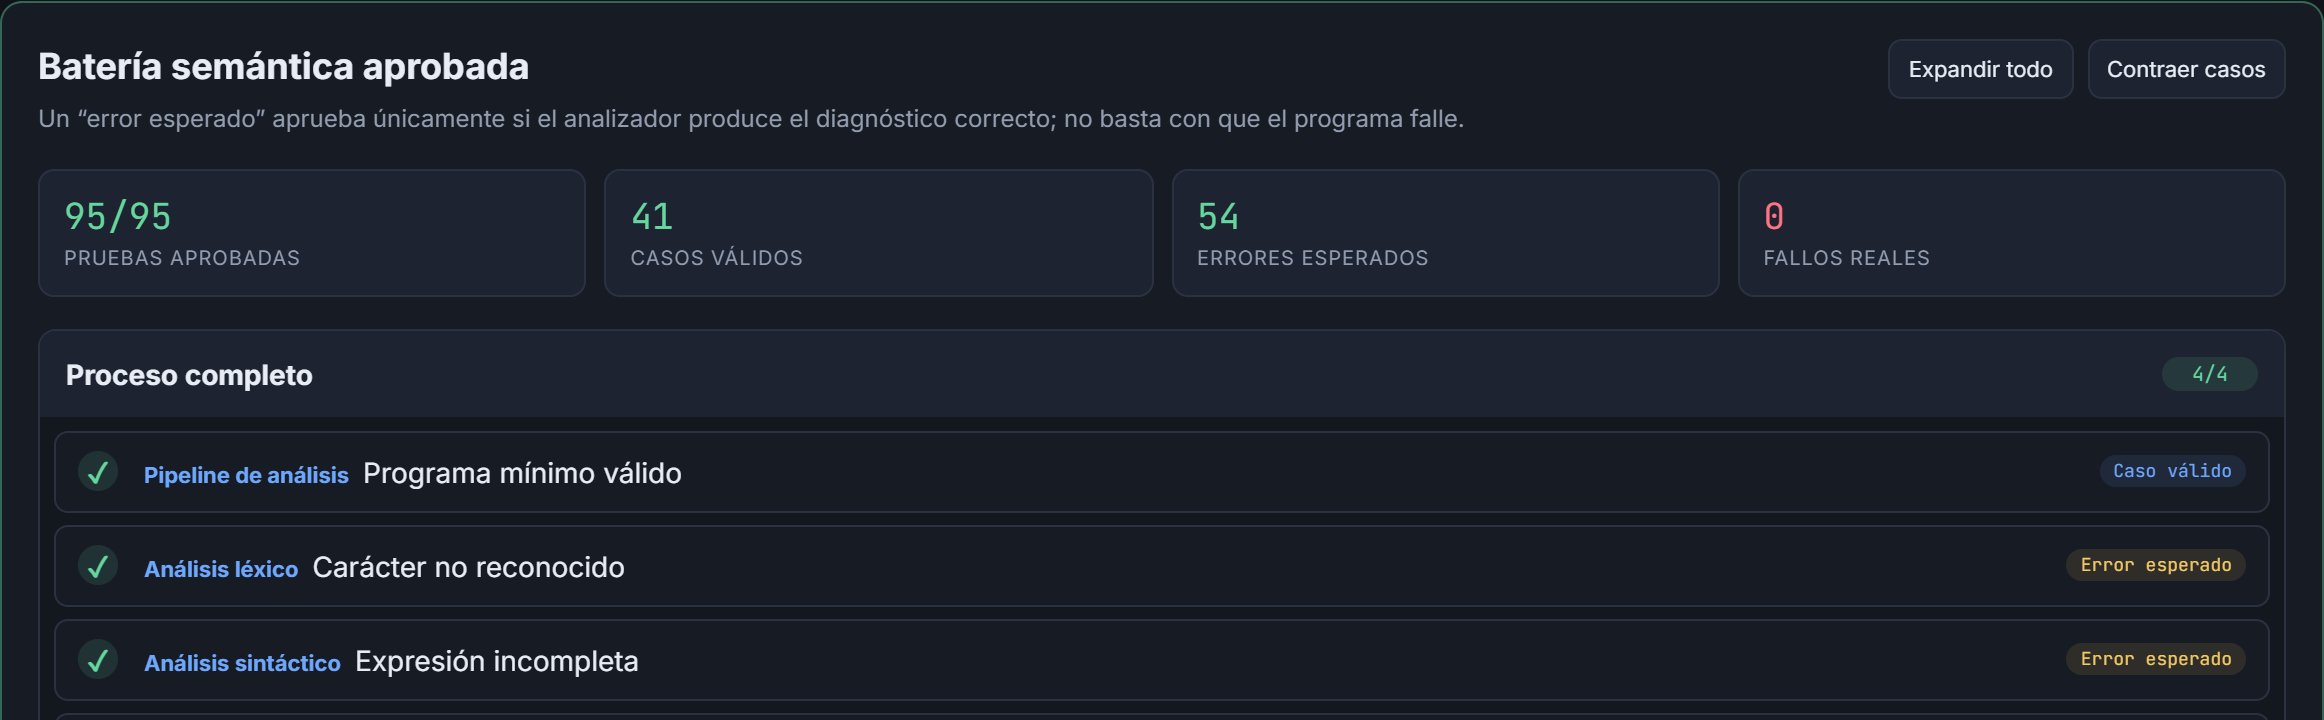
\includegraphics[width=\textwidth]{img/pruebas.png}
\caption{Batería ejecutada desde el IDE: 95/95, con 41 casos válidos, 54
errores esperados y 0 fallos reales.}
\end{figure}

La batería también puede ejecutarse desde la línea de comandos:

\begin{lstlisting}[language=bash,caption={Ejecución desde CTest.}]
ctest --test-dir build/compiscript --output-on-failure
\end{lstlisting}

% --------------------------------------------------- 11 CÓMO EJECUTARLO
\section{Compilación y ejecución}

\subsection{Requisitos}

\begin{itemize}[leftmargin=1.4em]
  \item CMake 3.20 o superior.
  \item Compilador compatible con C++17.
  \item Java, únicamente para ejecutar la herramienta generadora de ANTLR.
  \item Python 3 con Flask, únicamente para servir el IDE.
\end{itemize}

\subsection{Construcción}

Un solo script descarga el JAR oficial de ANTLR si hace falta, regenera el
lexer, el parser y el Visitor, descarga y compila el runtime C++ de ANTLR,
construye \texttt{compiscript\_cli} y \texttt{compiscript\_tests}, y ejecuta la
batería:

\begin{lstlisting}[language=bash,caption={macOS o Linux.}]
python3 -m pip install -r requirements.txt
./scripts/build_compiscript.sh
\end{lstlisting}

\begin{lstlisting}[language=bash,caption={Windows PowerShell.}]
python -m pip install -r requirements.txt
powershell -File scripts/build_compiscript.ps1
\end{lstlisting}

\subsection{Ejecución del IDE}

\begin{lstlisting}[language=bash,caption={Servidor del IDE.}]
python app.py
\end{lstlisting}

El IDE queda disponible en \texttt{http://127.0.0.1:5050}.

\subsection{Uso directo del CLI}

\begin{lstlisting}[language=bash,caption={Análisis desde la línea de comandos.}]
./compiscript_cli --file backend/examples/compiscript/bienvenido.cps
./compiscript_cli --stdin program.cps < program.cps
\end{lstlisting}

La salida es un único documento JSON. El código de salida es \texttt{0} cuando
no hay errores, \texttt{1} cuando el programa contiene diagnósticos y
\texttt{2} cuando el uso del CLI o el archivo de entrada no son válidos.

% ------------------------------------------------------- 12 DECISIONES
\section{Decisiones sobre el material oficial}

El enunciado, la especificación y la gramática entregada no coinciden entre sí
en tres puntos. Se resolvieron sin retirar construcciones oficiales.

\begin{itemize}[leftmargin=1.4em]
  \item \textbf{Se agregó \texttt{float}.} La rúbrica exige operaciones entre
        \texttt{integer} y \texttt{float}, pero la gramática base solo contiene
        enteros. La gramática activa añade el tipo, el literal decimal y la
        ampliación implícita \texttt{integer} $\rightarrow$ \texttt{float}.
  \item \textbf{\texttt{+} acepta dos \texttt{string}.} Los ejemplos oficiales
        usan concatenación. No se permite, en cambio, concatenar implícitamente
        cualquier objeto con un string.
  \item \textbf{Los cuerpos de control aceptan bloque o una sola sentencia.} El
        ejemplo oficial de recursión usa \texttt{if (n <= 1) return 1;} sin
        llaves, mientras la gramática base exigía bloque.
\end{itemize}

Existe además una contradicción explícita: la rúbrica exige que la condición de
\texttt{switch} sea \texttt{boolean}, mientras que el documento de ejemplos usa
un selector \texttt{integer}. \textbf{La implementación prioriza la regla
explícita de la rúbrica.} La comprobación de compatibilidad de los casos está
separada de la comprobación del selector, de modo que revertir esta decisión
requiere retirar una sola llamada a \texttt{requireType}.

Por coherencia con la misma regla, \texttt{break} dentro de un \texttt{switch}
que no está en un bucle también se reporta, porque el enunciado limita
\texttt{break} y \texttt{continue} a bucles.

% --------------------------------------------------------- 13 RÚBRICA
\section{Correspondencia con la rúbrica}

\begin{table}[H]
\centering
\small
\begin{tabular}{@{}L{4.0cm}rL{8.6cm}@{}}
\toprule
\textbf{Componente} & \textbf{Pts} & \textbf{Evidencia en el proyecto} \\
\midrule
IDE & 15 &
Editor con carga, guardado y descarga de \texttt{.cps}, análisis bajo demanda,
diagnósticos navegables y siete paneles de resultados. \\
\addlinespace
Analizador sintáctico y semántico & 60 &
Gramática y código generado por ANTLR con \emph{target} C++, árbol sintáctico
visual, Visitor semántico de 1\,218 líneas con 32 códigos de diagnóstico y
batería de 95 escenarios. \\
\addlinespace
Tabla de símbolos & 25 &
Símbolos y scopes enlazados por identificador estable, resolución por cadena de
ámbitos, registro de capturas de closures y vistas jerárquica y tabular por
entorno. \\
\midrule
\textbf{Total} & \textbf{100} & \\
\bottomrule
\end{tabular}
\caption{Evidencia por componente evaluado.}
\end{table}

Respecto a los entregables solicitados: el repositorio conserva commits
individuales por integrante (sección 4), la batería de pruebas cubre casos
exitosos y fallidos de cada regla semántica (sección 10), la arquitectura y las
instrucciones de ejecución están documentadas (secciones 3 y 11, además de
\texttt{docs/arquitectura-compiscript.md} y \texttt{README.md}), y el IDE es
funcional (sección 9).

% ---------------------------------------------------- 14 CONCLUSIONES
\section{Conclusiones}

\begin{enumerate}[leftmargin=1.6em]
  \item Mantener un único núcleo C++ consumido por el CLI, las pruebas y el
        servidor web eliminó la posibilidad de que la interfaz y la batería
        midieran comportamientos distintos. Es la decisión de diseño que más
        simplificó la depuración.

  \item El patrón Visitor resultó adecuado para el análisis semántico porque
        permite sintetizar el tipo de una expresión desde sus subexpresiones,
        devolviéndolo hacia el nodo padre. Con un Listener habría sido necesario
        administrar manualmente una pila de resultados.

  \item Conservar los scopes después de salir de cada bloque, en lugar de
        destruirlos, convirtió la tabla de símbolos en una instantánea completa
        y navegable del programa. Esto no solo satisface la evaluación: es la
        estructura que las fases posteriores del compilador necesitarán.

  \item Suspender el análisis semántico cuando hay errores sintácticos evita
        diagnósticos en cascada sobre un árbol incompleto, sin perder la
        información útil, porque los tokens y el árbol se siguen entregando.

  \item Las contradicciones entre el enunciado, la especificación y la gramática
        entregada obligaron a tomar decisiones explícitas. Documentarlas y
        aislarlas en el código ---el caso de \texttt{switch} se revierte
        retirando una sola llamada--- resultó más valioso que elegir en
        silencio.
\end{enumerate}

% ---------------------------------------------------- 15 REFERENCIAS
\section{Referencias}

\sloppy
\begin{itemize}[leftmargin=1.4em]
  \item Aho, A., Lam, M., Sethi, R. y Ullman, J. \emph{Compilers: Principles,
        Techniques, and Tools}. 2.\textsuperscript{a} edición, 2006.
        Secciones 2.7 (tablas de símbolos), 6.5 (comprobación de tipos) y 7.3
        (acceso a datos no locales).
  \item Parr, T. \emph{The Definitive ANTLR 4 Reference}. Documentación del
        \emph{target} de C++: \url{https://github.com/antlr/antlr4}.
  \item Enunciado del proyecto: \emph{Análisis Semántico de Compiscript},
        Construcción de Compiladores, agosto de 2026.
  \item Documentación interna del repositorio:
        \texttt{docs/arquitectura-compiscript.md} y
        \texttt{docs/decisiones-compiscript.md}.
\end{itemize}

\end{document}
